\documentclass{article}

% Encoding & fonts
\usepackage[T1]{fontenc}
\usepackage[utf8]{inputenc}
\usepackage{lmodern}

\usepackage{graphicx}
\usepackage{enumitem} 
\usepackage{float}
\usepackage{booktabs}
\usepackage{multirow}
\usepackage{longtable}
\usepackage{array}


\usepackage{amsmath, amssymb, amsfonts}
\usepackage[a4paper,margin=3cm]{geometry}
\usepackage{tikz}
\usetikzlibrary{shapes.geometric, arrows.meta, positioning, shadows, calc, fit, backgrounds}
\usepackage{xcolor}

% Define custom colors
\definecolor{scenarioBlue}{RGB}{52, 152, 219}
\definecolor{milpRed}{RGB}{231, 76, 60}
\definecolor{graphGreen}{RGB}{46, 204, 113}
\definecolor{encoderPurple}{RGB}{155, 89, 182}
\definecolor{ebmOrange}{RGB}{243, 156, 18}
\definecolor{samplerTeal}{RGB}{26, 188, 156}
\definecolor{decoderPink}{RGB}{233, 30, 99}
\definecolor{lpworkerBrown}{RGB}{121, 85, 72}
\definecolor{evalGray}{RGB}{96, 125, 139}
\definecolor{bgLight}{RGB}{248, 249, 250}

% ==== BIBLIO: BibTeX + natbib (auteur–année) ====
\usepackage[round,authoryear]{natbib}

% (Optionnel) compat si tu as déjà beaucoup de \parencite dans le texte
\let\parencite\citep

% Hyperlinks (load after natbib)
\usepackage[hidelinks]{hyperref}


\title{Coordinating Multilayer Power System Flexibility:\\
A Hybrid MILP--GNN--EBM Framework for Large-Scale Scenario Exploration}
\author{Théotime Coudray* \\ Stéphane Goutte*\\[2pt]
\normalsize *Université de Versailles Saint-Quentin-en-Yvelines (UVSQ), UMI SOURCE}
\date{}

\begin{document}

\maketitle

\begin{abstract}
Power-system flexibility studies increasingly demand \emph{scenario exploration} rather than single-shot optimisation: analysts must evaluate large ensembles of ``what-if'' cases that combine multi-scale resources (storage, demand response, inter-area exchanges), network limits, evolving topology, and correlated uncertainty. Mixed-integer linear programming (MILP) provides rigorous and auditable answers, but repeated solves quickly become prohibitive as scenario volume and complexity grow. We propose a hybrid \textbf{MILP--GNN--EBM} methodology designed for near-real-time exploration. A multi-layer MILP oracle is first solved on a diversity-maximising scenario set to generate optimal labels. Each instance is then represented as a heterogeneous temporal graph and processed by a topology-consistent graph neural network (GNN) that produces compact scenario embeddings. Conditioned on these embeddings, an energy-based model (EBM) learns an energy landscape over binary activation/commitment decisions and enables fast sampling of multiple high-quality candidates via Langevin dynamics. A lightweight feasibility decoder repairs residual violations, and a conditional LP worker recovers the continuous dispatch to produce complete, economically meaningful operating plans. We evaluate speed, feasibility, and optimality across scenario families of increasing difficulty, testing whether the MILP--GNN--EBM stack provides larger benefits as scenarios become more complex.
\end{abstract}

\noindent\textbf{Keywords:} Power System; Multi-Scale Modelling; MILP; Graph Neural Networks; Energy-Based Models; Scenario Exploration.

\section{Introduction}

Power systems are undergoing a profound transformation, driven by the large-scale integration of variable renewable energy (VRE), rapid electrification of end uses, and the growing penetration of distributed energy resources (DER) such as demand response (DR) and storage. This transition pushes system operators and planners to mobilize flexibility across \emph{multiple spatial layers} (from behind-the-meter assets to regional and national transmission systems) and \emph{multiple temporal scales} (from intra-hour balancing to seasonal adequacy), while guaranteeing feasibility under network, market, and security constraints.

A central methodological challenge is that the questions stakeholders increasingly ask are not single-run questions (``what is the optimal schedule today?''), but \emph{interactive what-if questions} that require exploring thousands of scenarios: extreme weather and correlated forecast errors, congestion and topology changes, new flexibility portfolios (storage and DR), and coupled infrastructures (e.g., gas--power--carbon interactions). In these settings, the practical bottleneck is not only solving one high-fidelity instance, but enabling \emph{near-real-time scenario exploration} where users can turn a ``complexity knob'' (more spatial detail, longer horizons, tighter constraints, more uncertainty) and still obtain fast, credible answers.

Mixed-Integer Linear Programming (MILP) provides a rigorous and auditable representation of these decisions, and remains the reference tool for high-fidelity scheduling and planning \parencite{conejo_investment_2016}. However, repeated MILP solves become rapidly prohibitive as scenario count and model complexity increase, due to non-convexities (e.g., unit commitment logic) and strong inter-temporal and network couplings. Conversely, learning-based surrogates---and in particular Graph Neural Networks (GNNs)---can exploit grid topology to deliver fast predictions, but purely predictive approaches can violate hard constraints, drift out of distribution, and lose economic meaning.

This paper proposes a hybrid \textbf{MILP--GNN--EBM methodology for multi-scale flexibility exploration} that turns high-fidelity optimization into an exploration engine. Concretely, we propose an end-to-end pipeline that couples synthetic scenario generation, a multi-layer MILP oracle, topology-consistent graph representations, and learning-based inference with feasibility-preserving post-processing.

Rather than replacing optimization, the proposed surrogate stack aims to preserve MILP-level structure while enabling \emph{near-real-time} scenario sweeps: the MILP produces ground truth, the GNN compresses scenarios into informative representations, the EBM provides controlled exploration over binaries, and the decoder+LP stages restore feasibility and compute the final dispatch. The objective is not to predict a single optimal solution, but to enable fast and controlled exploration of high-quality feasible solutions as scenario complexity increases.


\subsection{Literature Review}

MILP remains the workhorse for operational scheduling (e.g., unit commitment and multi-period dispatch) and long-term planning under uncertainty, due to its ability to encode discrete decisions, operational constraints, and economic objectives in a transparent manner \parencite{conejo_investment_2016}. In expansion planning, stochastic and multi-stage MILP formulations capture uncertainty in costs and renewable availability, but typically require decomposition, scenario reduction, or aggregation to remain tractable \parencite{micheli_two-stage_2023}. Beyond single-level optimization, multi-level and equilibrium-aware formulations have been developed to represent strategic interactions and sequential market clearings: early MPEC-based approaches model strategic bidding under network constraints \parencite{hobbs_strategic_2000}, while three-level MILP formulations integrate transmission expansion, generation investment, and market equilibrium at the operational layer \parencite{pozo_three-level_2013}. More recently, scalable approximations for mixed-integer multi-level problems with sequential followers have been proposed, together with dedicated Benders-type decomposition strategies to address computational scaling in coupled electricity--gas--carbon market settings \parencite{xia_scalable_2025}.

Building on these MILP foundations, when flexibility is distributed across buildings, districts, and regions, MILP models can explicitly represent coordination across spatial layers, but the number of integer variables and coupling constraints grows rapidly with resolution and horizon length. Holarchic or hierarchical formulations mitigate this growth through structured aggregation and decomposition, enabling urban- or district-scale optimization while preserving key network interactions \parencite{marquant_holarchic_2017}. Robust hierarchical MILP designs further address uncertainty (e.g., demand ranges) via min--max constructs, at the cost of additional layers and higher computational burden \parencite{yokoyama_hierarchical_2021}. Overall, the literature shows a consistent tension: high-fidelity multi-layer MILPs are auditable and economically meaningful, but they remain expensive for large scenario sweeps and interactive exploration.

To alleviate this computational bottleneck, recent work has explored GNNs as topology-aware surrogates or accelerators. Early work showed that graph neural architectures can emulate load-flow/physics solvers and generalize across topologies \parencite{donon_graph_2019}, and can approximate OPF solutions via imitation learning on AC settings \parencite{owerko_optimal_2019}. For AC optimal power flow (AC-OPF), topology-informed GNNs have been designed with feasibility regularization and adaptation mechanisms for topology contingencies \parencite{liu_topology-aware_2023}. Complementary approaches use GNNs to provide warm-starts or initial estimates, reducing the iteration count of interior-point solvers and thereby accelerating high-fidelity OPF computations \parencite{deihim_initial_2024}. Other studies benchmark GNN architectures (e.g., attention-based) for efficient AC power flow or OPF prediction in larger grids \parencite{talebi_graph_2025}. Beyond OPF, GNN proxies have been trained from large collections of MILP solves to support hours-ahead risk assessment under evolving topology, with reported gains in speed and situational awareness \parencite{zhang_graph_2024}. In restoration and UC-like settings, learning-based policies have also been proposed to accelerate MILP-based decision making, e.g., for load restoration \parencite{ahmed_advancing_2024}, by predicting an initial commitment refined via large neighborhood search \parencite{yang_solving_nodate}, or by directly learning branching/diving policies in modern MIP solvers \parencite{qin_solve_2023}. Related hybrid strategies combine GNN predictions with LP relaxations to fix stable variables and accelerate UC while controlling suboptimality \parencite{yang_stable_2025}, and confidence-aware architectures seed commitment and active-constraint predictions to speed up large industrial RAC formulations \parencite{park_confidence-aware_2023}. At the planning level, GNN surrogates have been proposed to approximate the outputs of MILP energy system models, enabling faster what-if analyses \parencite{pjetri_graph_nodate}.

A persistent challenge in learning-to-optimize is enforcing hard constraints and providing controlled exploration of complex discrete spaces. Two complementary strands are particularly relevant: (i) learning to make discrete decisions inside MILP solvers, and (ii) learning generative/energy-based models for exploration.

On the solver side, MILPs admit a natural bipartite constraint--variable graph representation that can be exploited by GNN policies for branching decisions \parencite{gasse_exact_2019}. However, fundamental representational limits also exist: there are MILP families that all GNNs will treat equally unless additional structure or features are injected \parencite{chen_representing_2023}, motivating hybrid designs where learning is guided by optimization structure.

On the generative side, energy-based formulations offer a principled bridge: combinatorial objectives can be written as energies, and neural networks can be trained to approximate these energies and sample high-quality solutions. In particular, annealed training has been proposed to cast graph combinatorial optimization problems as unbiased EBMs with carefully selected penalties, yielding more stable unsupervised training and improved solution quality \parencite{sun_annealed_2022}. Progress in discrete sampling benchmarks further highlights the importance of robust, scalable samplers for discrete/structured distributions \parencite{goshvadi_discs_2023}. EBMs have also been explored for non-convex, cardinality-constrained portfolio optimization, illustrating GPU-accelerated sampling as an alternative to single-solution pipelines \parencite{mancilla_non-convex_2026}.

In parallel, differentiable satisfiability and projection layers have been developed to enforce general linear constraints (including those arising in unit commitment), offering end-to-end differentiable mechanisms to project neural outputs back into feasible sets \parencite{zeng_glinsat_2024}. When scenario exploration involves composite and time-varying action spaces (e.g., heterogeneous flexibility levers becoming available/unavailable), structured cooperative RL provides additional design patterns for handling such changing decision sets \parencite{li_structured_2021}. More broadly, generator-enhanced optimization frameworks leverage generative models (classical or quantum-inspired) to improve search-space exploration for hard optimization problems \parencite{alcazar_enhancing_2024}.

\subsection{Research Gap and Research Statement}

\begin{enumerate}[label=\textbf{(\arabic*)}, leftmargin=*, itemsep=2pt]
  \item \emph{Scenario exploration at scale is still solver-bound.} Multi-layer and multi-level MILP formulations remain too costly to support near-real-time exploration when the number of scenarios grows (stress cases, coupled markets, topology changes), despite decomposition and aggregation strategies \parencite{micheli_two-stage_2023,pozo_three-level_2013,xia_scalable_2025,marquant_holarchic_2017}.
  \item \emph{Learning surrogates rarely deliver end-to-end feasibility across layers.} GNN surrogates can be accurate and topology-aware for specific tasks (OPF, risk assessment, restoration), yet guaranteeing feasibility across heterogeneous layers (assets--zones--regions) and across long horizons remains difficult without an explicit feasibility mechanism \parencite{liu_topology-aware_2023,zhang_graph_2024,ahmed_advancing_2024}.
  \item \emph{Limited support for controlled exploration under increasing scenario complexity.} Existing surrogates are often trained for prediction; fewer approaches explicitly address exploration of large discrete decision spaces (commitment logic, discrete DR activation) in a way that remains robust as scenario complexity increases \parencite{yang_solving_nodate,sun_annealed_2022,goshvadi_discs_2023}.
  \item \emph{Weak coupling between economic signals and learned inference.} Multi-level/equilibrium MILP models yield meaningful price signals and strategic interactions, but most learning pipelines do not exploit this structure to steer inference or sampling toward economically consistent solutions \parencite{hobbs_strategic_2000,pozo_three-level_2013,xia_scalable_2025}.
  \item \emph{From point predictions to interactive, near-real-time what-if analysis.} Warm-starting and surrogate prediction accelerate single runs, but the literature provides limited methodology for interactive, user-driven scenario sweeps where the ``complexity knob'' (spatial detail, coupling, uncertainty, topology changes) is increased while preserving speed, feasibility, and interpretability \parencite{deihim_initial_2024,pjetri_graph_nodate,talebi_graph_2025}.
\end{enumerate}

\paragraph{}
The central research question is therefore:
\emph{Can a hybrid MILP--GNN--EBM methodology enable near-real-time exploration of multi-scale flexibility scenarios---and remain effective as scenarios become increasingly complex (heterogeneous layers, discrete decisions, uncertainty, and topology change)?}

\subsection{Contributions}
Our main contributions are:
\begin{enumerate}[label=\textbf{C\arabic*}, leftmargin=*, itemsep=2pt]
  \item \textbf{A flexibility scenario generator with diversity maximisation and complexity indexing.} We sample a wide range of techno-economic parameters to maximise scenario diversity and compute a scenario-specific complexity indicator that ranks instances by expected difficulty.
  \item \textbf{A multi-layer MILP oracle for coordinated flexibility.} We formulate and solve a high-fidelity MILP that coordinates multi-scale flexibility resources under network and inter-temporal constraints, producing auditable primal schedules (and optional dual signals).
  \item \textbf{A projection of scenario instances to hierarchical multi-layer temporal graphs.} Each scenario is encoded as a heterogeneous temporal graph that mirrors the nested physical/aggregation structure (assets $\to$ zones $\to$ regions $\to$ system) while preserving time-coupled constraints.
  \item \textbf{A topology-consistent GNN encoder for scenario embeddings.} We learn a GNN encoder that captures scenario structure and maps each instance into an embedding space that preserves the hierarchical, multi-layer, and temporal organisation of the system.
  \item \textbf{A graph EBM sampler with feasibility-preserving decoding.} Conditioned on scenario embeddings, an EBM learns an energy landscape over binary decisions and enables fast sampling; a lightweight decoder repairs residual violations, and a conditional LP worker recovers continuous dispatch.
  \item \textbf{An evaluation protocol for large-scale scenario exploration.} We quantify speed, feasibility, and optimality across scenario families of increasing complexity, testing how performance evolves as the exploration ``complexity knob'' is increased.
\end{enumerate}

\subsection{Paper Organization}
The remainder of this paper is organized as follows. Section~2 introduces the overall pipeline and details the scenario generation process and the multi-layer MILP oracle used to produce optimal labels for training. Section~3 presents the hierarchical heterogeneous temporal graph representation and the topology-consistent encoder that maps each scenario to compact embeddings. Section~4 describes the conditional graph EBM and the Langevin-based sampling strategy for discrete decision candidates. Section~5 is dedicated to the post-processing stages that restore feasibility and recover continuous dispatch through a feasibility decoder and an LP worker. Section~6 discusses the experimental setup, including datasets, evaluation metrics, and the protocol to compare runtime, feasibility, and optimality between families of scenarios with increasing complexity. This section also presents the main results, with a particular focus on how performance evolves as the scenario ``complexity knob'' is increased. Finally, Section~7 concludes and outlines the current limitations and directions for future work, including security constraints, uncertainty extensions, and deployment-oriented robustness mechanisms.


\section{Methodology Overview and Training Data Generation}
Figure~\ref{fig:milp-gnn-ebm-pipeline} presents the proposed MILP--GNN--EBM pipeline as an end-to-end exploration engine that transforms high-fidelity optimization into fast and controllable large-scale scenario sweeps. Starting from a broad pool of synthetic what-if cases, the workflow proceeds as follows: (i) we generate a diversity-maximizing set of scenarios and compute for each of them a scenario-level complexity index capturing combinatorial and operational stress; (ii) a multi-layer MILP oracle is solved to produce optimal solutions; (iii) each instance is projected onto a hierarchical, heterogeneous temporal graph and encoded via a topology-consistent GNN into a compact latent representation; (iv) a conditional graph EBM is trained to efficiently explore the space of high-quality discrete decisions; (v) candidate solutions are then repaired and completed through a feasibility-aware decoder and a conditional LP worker to recover continuous dispatch variables; finally, (vi) the resulting solutions are benchmarked with scenario families of increasing complexity against the pure MILP oracle in terms of runtime, feasibility rate, and cost optimality gap.


\begin{figure}[p]
\centering

\resizebox{\textwidth}{!}{%
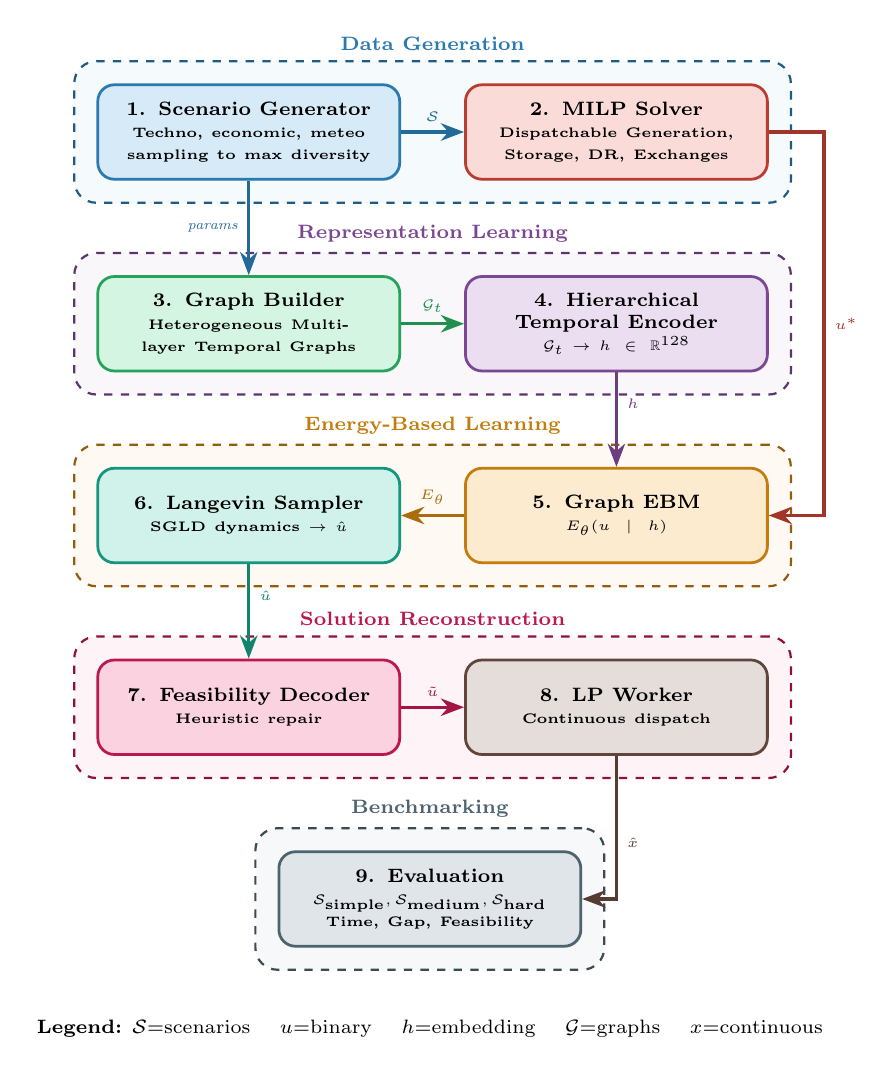
\begin{tikzpicture}[
    % Node styles
    block/.style={
        rectangle,
        rounded corners=6pt,
        minimum width=3.8cm,
        minimum height=1.2cm,
        text centered,
        text width=3.6cm,
        font=\scriptsize\bfseries,
        draw=#1!80!black,
        fill=#1!20,
        line width=1pt,
        drop shadow={shadow xshift=0.5pt, shadow yshift=-0.5pt, opacity=0.2}
    },
    % Arrow style
    arrow/.style={
        ->,
        >=Stealth,
        line width=1.2pt,
        draw=#1!70!black
    },
    % Data flow annotation style
    annot/.style={
        font=\tiny\itshape,
        text=#1!70!black,
        align=center
    },
    % Group box style
    groupbox/.style={
        draw=#1!60!black,
        fill=#1!5,
        rounded corners=8pt,
        line width=0.8pt,
        dashed
    }
]

% ============================================
% ROW 1: DATA GENERATION
% ============================================
% Scenario Generator
\node[block=scenarioBlue] (generator) {
    \textbf{1. Scenario Generator}\\
    \tiny Techno, economic, meteo sampling to max diversity
};

% MILP Solver (right of generator)
\node[block=milpRed, right=0.8cm of generator] (milp) {
    \textbf{2. MILP Solver}\\
    \tiny Dispatchable Generation, Storage, DR, Exchanges
};

% ============================================
% ROW 2: REPRESENTATION LEARNING
% ============================================
% Graph Construction
\node[block=graphGreen, below=1.2cm of generator] (graphs) {
    \textbf{3. Graph Builder}\\
    \tiny Heterogeneous Multilayer Temporal Graphs
};

% Hierarchical Encoder
\node[block=encoderPurple, right=0.8cm of graphs] (encoder) {
    \textbf{4. Hierarchical Temporal Encoder}\\
    \tiny $\mathcal{G}_t$ $\rightarrow$ $h \in \mathbb{R}^{128}$
};

% ============================================
% ROW 3: ENERGY-BASED LEARNING
% ============================================
% EBM Training
\node[block=ebmOrange, below=1.2cm of encoder] (ebm) {
    \textbf{5. Graph EBM}\\
    \tiny $E_\theta(u \mid h)$
};

% Langevin Sampler
\node[block=samplerTeal, left=0.8cm of ebm] (sampler) {
    \textbf{6. Langevin Sampler}\\
    \tiny SGLD dynamics $\rightarrow$ $\hat{u}$
};

% ============================================
% ROW 4: SOLUTION RECONSTRUCTION
% ============================================
% Feasibility Decoder
\node[block=decoderPink, below=1.2cm of sampler] (decoder) {
    \textbf{7. Feasibility Decoder}\\
    \tiny Heuristic repair
};

% LP Worker
\node[block=lpworkerBrown, right=0.8cm of decoder] (lpworker) {
    \textbf{8. LP Worker}\\
    \tiny Continuous dispatch
};

% ============================================
% ROW 5: EVALUATION
% ============================================
% Evaluation (centered)
\node[block=evalGray, below=1.2cm of decoder, xshift=2.3cm] (eval) {
    \textbf{9. Evaluation}\\
    \tiny $\mathcal{S}_{\text{simple}}, \mathcal{S}_{\text{medium}}, \mathcal{S}_{\text{hard}}$ Time, Gap, Feasibility
};

% ============================================
% ARROWS - Main Flow
% ============================================

% Generator -> MILP
\draw[arrow=scenarioBlue] (generator.east) -- (milp.west)
    node[annot=scenarioBlue, midway, above] {$\mathcal{S}$};

% Generator -> Graphs
\draw[arrow=scenarioBlue] (generator.south) -- (graphs.north)
    node[annot=scenarioBlue, midway, left] {params};

% MILP -> Graph EBM (optimal solutions)
\draw[arrow=milpRed] (milp.east) -- ++(0.7,0cm) |- (ebm.east)
    node[annot=milpRed, pos=0.25, right] {$u^*$};

% Graphs -> Encoder
\draw[arrow=graphGreen] (graphs.east) -- (encoder.west)
    node[annot=graphGreen, midway, above] {$\mathcal{G}_t$};

% Encoder -> EBM
\draw[arrow=encoderPurple] (encoder.south) -- ++(0,-0.4cm) -| (ebm.north)
    node[annot=encoderPurple, pos=0.25, right] {$h$};

% EBM -> Sampler
\draw[arrow=ebmOrange] (ebm.west) -- (sampler.east)
    node[annot=ebmOrange, midway, above] {$E_\theta$};

% Sampler -> Decoder
\draw[arrow=samplerTeal] (sampler.south) -- ++(0,-0.4cm) -| (decoder.north)
    node[annot=samplerTeal, pos=0.25, right] {$\hat{u}$};

% Decoder -> LP Worker
\draw[arrow=decoderPink] (decoder.east) -- (lpworker.west)
    node[annot=decoderPink, midway, above] {$\tilde{u}$};

% LP Worker -> Eval
\draw[arrow=lpworkerBrown] (lpworker.south) -- ++(0,-0.4cm) |- (eval.east)
    node[annot=lpworkerBrown, pos=0.25, right] {$\hat{x}$};


% ============================================
% PHASE LABELS (Background boxes)
% ============================================
\begin{scope}[on background layer]
    % Data Generation phase
    \node[groupbox=scenarioBlue, fit=(generator)(milp), inner sep=8pt, 
          label={[font=\scriptsize\bfseries, scenarioBlue!80!black]above:Data Generation}] {};
    
    % Representation Learning phase
    \node[groupbox=encoderPurple, fit=(graphs)(encoder), inner sep=8pt,
          label={[font=\scriptsize\bfseries, encoderPurple!80!black]above:Representation Learning}] {};
    
    % Energy-Based Learning phase
    \node[groupbox=ebmOrange, fit=(ebm)(sampler), inner sep=8pt,
          label={[font=\scriptsize\bfseries, ebmOrange!80!black]above:Energy-Based Learning}] {};
    
    % Solution Reconstruction phase
    \node[groupbox=decoderPink, fit=(decoder)(lpworker), inner sep=8pt,
          label={[font=\scriptsize\bfseries, decoderPink!80!black]above:Solution Reconstruction}] {};
    
    % Evaluation phase
    \node[groupbox=evalGray, fit=(eval), inner sep=8pt,
          label={[font=\scriptsize\bfseries, evalGray!80!black]above:Benchmarking}] {};
\end{scope}

% ============================================
% LEGEND
% ============================================
\node[below=0.8cm of eval, xshift=0cm] (legend) {
    \scriptsize\textbf{Legend:} $\mathcal{S}$=scenarios \quad $u$=binary \quad $h$=embedding \quad $\mathcal{G}$=graphs \quad ${x}$=continuous
};

\end{tikzpicture}
}

\vspace{0.6em}

\small
\begin{tabular}{clll}
\toprule
\textbf{\#} & \textbf{Component} & \textbf{Input} & \textbf{Output} \\
\midrule
1 & Scenario Generator & Parameter distributions & Diverse scenarios $\mathcal{S}$ \\
2 & MILP Solver & Scenarios $\mathcal{S}$ & Optimal decisions $(u^*, x^*)$ \\
3 & Graph Builder & Scenarios $\mathcal{S}$ & Heterogeneous temporal graphs $\mathcal{G}_t$ \\
4 & Hierarchical Encoder & Graphs $\mathcal{G}_t$ & Embeddings $h \in \mathbb{R}^{128}$ \\
5 & Graph EBM & $(u^*, h)$ pairs & Energy function $E_\theta(u \mid h)$ \\
6 & Langevin Sampler & $E_\theta$ & Candidate binaries $\hat{u}$ \\
7 & Feasibility Decoder & $\hat{u}$ & Feasible binaries $\tilde{u}$ \\
8 & LP Worker & $\tilde{u}$ & Continuous dispatch $\hat{x}$ \\
9 & Evaluation & Pipeline vs MILP outputs & Time, gap, feasibility \\
\bottomrule
\end{tabular}


\caption{Flow chart and module summary of the proposed hybrid MILP–GNN–EBM framework.}
\label{fig:milp-gnn-ebm-pipeline}
\end{figure}



% ============================================================
% SECTION 2.1: SCENARIO GENERATOR
% ============================================================

\subsection{Scenario Generator}
\label{sec:scenario_generator}

The first stage of our pipeline is a \emph{synthetic scenario generator} that produces a diverse set of power-system flexibility instances to train and evaluate the downstream learning modules. Each scenario encodes a complete specification of the system: network topology, asset portfolio, economic policies, technical constraints, and exogenous drivers (weather, demand, hydro inflows). The generator is designed to (i)~span a wide range of physical stress levels and combinatorial hardness, (ii)~remain computationally tractable for MILP labelling, and (iii)~avoid redundant near-duplicate instances that waste compute budget.

\subsubsection{Scenario Parameter Space}
\label{sec:scenario_space}

A scenario $s$ is fully characterized by a configuration tuple
\begin{equation}
s = \bigl(\mathcal{G}, \mathcal{A}, \pi, \tau, c, \xi\bigr),
\end{equation}
where $\mathcal{G}$ is the network graph, $\mathcal{A}$ is the asset specification, $\pi$ denotes economic policy parameters, $\tau$ collects technical scalers, $c$ represents operation costs, and $\xi$ captures exogenous drivers.

\paragraph{Network structure $\mathcal{G}$.}
The spatial hierarchy follows a \emph{assets $\rightarrow$ zones $\rightarrow$ regions $\rightarrow$ nation} structure. For each scenario we sample:
\begin{itemize}[noitemsep]
  \item number of regions $|\mathcal{R}|$,
  \item zones per region $|\mathcal{Z}_r|$ (sampled independently per region),
  \item assets are sampled either at the zone level ($|\mathcal{A}_z$|) or at the region level ($|\mathcal{A}_r$|), depending on the technology (e.g., nuclear units are regional, while solar units are zonal),
  \item intertie density $\rho$ controlling inter-regional transmission,
  \item number of neighbouring nations $|\mathcal{N}|$ for cross-border exchanges.
\end{itemize}

\paragraph{Asset portfolio $\mathcal{A}$.}
Asset counts are sampled at zone or regional level:
\begin{itemize}[noitemsep]
  \item thermal, run-of-river hydro, solar and wind units per zone,
  \item battery storage and demand-response resources per zone,
  \item nuclear plants, reservoir hydro and pumped-hydro storage per region
\end{itemize}

\paragraph{Economic policy $\pi$.}
Policy levers include CO$_2$ price (EUR/t), price cap (EUR/MWh), cross-border policy (free, limited, or blocked), and import/export caps.

\paragraph{Technical scalers $\tau$.}
Key flexibility drivers include thermal ramp rates, minimum generation ratios, battery energy-to-power ratio, round-trip efficiency, final state-of-charge tolerances, and demand-response parameters (max shed share, duration, number of activation events, ramp limits).

\paragraph{Exogenous drivers $\xi$.}
Weather and load conditions are captured by:
\begin{itemize}[noitemsep]
  \item a dominant weather profile (e.g., sunny summer, stormy winter, cloudy spring),
  \item per-region weather cells with profile and spread intensity,
  \item demand profile (weekday peak, weekend flat, etc.) and demand scale factor,
  \item hydro inflow factor.
\end{itemize}
To preserve spatial heterogeneity, each region draws its own weather profile; summary statistics (histogram, entropy, min/mean/max spread) are retained for diversity computation.

\subsubsection{Budget Guard}
\label{sec:budget_guard}

Not all randomly sampled scenarios are tractable within a fixed compute budget. Before acceptance, each candidate $s$ passes through a \emph{budget guard} that estimates MILP size and solve time:
\begin{equation}
\widehat{n}_{\mathrm{var}}(s) = f_{\mathrm{var}}(\mathcal{G}, \mathcal{A}, |\mathcal{T}|),
\end{equation}
where $|\mathcal{T}|$ is the number of time steps. A polynomial time estimator then predicts solve time:
\begin{equation}
\widehat{t}(s) = \beta_0 + \beta_1 \widehat{n}_{\mathrm{var}} + \beta_2 \widehat{n}_{\mathrm{cont}} + \beta_3 \widehat{n}_{\mathrm{bin}},
\end{equation}
where $\widehat{n}_{\mathrm{var}}$ is the estimated total number of decision variables,
$\widehat{n}_{\mathrm{cont}}$ the estimated number of continuous variables,
and $\widehat{n}_{\mathrm{bin}}$ the estimated number of binary variables
(unit commitment, nuclear commitment, and demand-response activation flags). Scenarios exceeding thresholds on variables, constraints, or predicted solve time are rejected.

\subsubsection{Diversity Maximization}
\label{sec:diversity}

Uniform random sampling tends to cluster in high-dimensional parameter space and over-represents ``easy'' instances. We employ two complementary strategies to maximize useful diversity.

\paragraph{Latin Hypercube Sampling (LHS).}
For continuous parameters that drive stress and difficulty (demand scale, inflow factor, CO$_2$ price, intertie density, ramp percentages, storage E/P ratio, import caps), we replace uniform sampling with Latin Hypercube Sampling. LHS partitions each marginal into $N$ equiprobable intervals and ensures exactly one sample per interval, yielding more uniform coverage in high dimensions. Compared to uniform random sampling, LHS reduces clustering and ensures better coverage of extreme parameter combinations.

\paragraph{Greedy $k$-center selection.}
Rather than accepting candidates online, we generate a large candidate pool (e.g., $20 \times$ target size) passing the budget guard, then select the final set via a greedy farthest-point algorithm:
\begin{equation}
s_{t+1} = \arg\max_{s \in \mathcal{P}} \min_{s' \in \mathcal{S}_t} d\bigl(v(s), v(s')\bigr),
\end{equation}
where $\mathcal{P}$ is the candidate pool, $\mathcal{S}_t$ is the selected set, and $v(s) \in \mathbb{R}^d$ is a normalized \emph{diversity vector} encoding topology, asset mix, technical scalers, and exogenous drivers. This ensures a minimum pairwise separation $d_{\min}$ and avoids near-duplicates. Intuitively, this procedure iteratively selects scenarios that are maximally dissimilar from those already selected, thereby spreading the final dataset over the diversity space and avoiding redundant instances.


\paragraph{}
LHS is applied at the parameter-sampling stage to ensure marginal coverage of key continuous drivers, while greedy $k$-center selection operates at the scenario level to enforce global diversity across structural, technical, and exogenous dimensions.

\paragraph{Stratification.}
To prevent over-representation of easy scenarios, we partition candidates into bins along stress and hardness axes (e.g., demand-scale quintiles, topology-size quartiles, weather-profile categories) and allocate quotas per bin before $k$-center selection. Stratification ensures that rare but operationally critical scenarios are sufficiently represented in the training set, rather than being drowned out by a majority of mild instances.


\subsubsection{Scenario Criticality Indicator}
\label{sec:criticality}

To characterize scenario difficulty \emph{ex ante} (before solving), we define a composite criticality indicator decomposed into physical stress and combinatorial hardness:
\begin{equation}
\mathrm{Crit}(s) = \alpha \, \mathrm{Stress}(s) + (1-\alpha) \, \mathrm{Hard}(s), \quad \alpha \in [0,1].
\end{equation}

All components of $\mathrm{Crit}(s)$ are computable ex ante, without solving the MILP.

\paragraph{Physical Stress Index.}
The stress component captures techno-operational tension through 12 normalized metrics grouped into four categories:
\begin{enumerate}[noitemsep, label=(\alph*)]
  \item \textbf{Variability:} VRE penetration ratio, residual-demand volatility, peak-to-valley ratio, short-term variability index.
  \item \textbf{Load level:} demand scale factor, peak-to-firm capacity ratio.
  \item \textbf{Flexibility margins (inverse):} storage power adequacy, storage energy adequacy, thermal flexibility ratio, DR headroom.
  \item \textbf{Spatial tension:} import/export reliance, congestion exposure proxy.
\end{enumerate}

\paragraph{Combinatorial Hardness Index.}
The hardness component captures structural MILP difficulty through 10 metrics:
\begin{enumerate}[noitemsep, label=(\alph*)]
  \item \textbf{Problem size:} number of zones $|\mathcal{Z}|$, horizon length $|\mathcal{T}|$, estimated binary count.
  \item \textbf{Non-convexity:} thermal unit density, minimum-generation tightness, startup-cost intensity.
  \item \textbf{Temporal coupling:} ramping tightness, SOC tightness proxy.
  \item \textbf{Spatial coupling:} interconnection density, network heterogeneity.
\end{enumerate}

\paragraph{}
These metrics were selected to jointly capture (i) known drivers of operational stress in power systems and (ii) structural sources of MILP hardness identified in the unit-commitment literature \parencite{buchheim_polytope_2023, huang_cutting_2021, morales_espana_tight_2013}. For completeness and reproducibility, Appendix~\ref{app:criticality} reports the definitions of the 22 metrics used to build the ex ante criticality index.


\paragraph{}
Each metric is normalized to $[0,1]$ using generator-bound scaling and combined as weighted sums:
\begin{equation}
\mathrm{Stress}(s) = \sum_{i=1}^{12} w_i^{(S)} \tilde{x}_i^{(S)}(s), \quad
\mathrm{Hard}(s) = \sum_{j=1}^{10} w_j^{(H)} \tilde{x}_j^{(H)}(s).
\end{equation}
The criticality index enables stratified sampling and post-hoc analysis of solver performance versus scenario difficulty.

    \paragraph{}
    Table~\ref{tab:scenario-comparison} and Figure~\ref{fig:scenario_figure} contrast a simple scenario (low criticality) with a critical one, illustrating the range of characteristics captured by the generator, as well as capacities and demand levels in these two instances.
    
    \begin{table}[htbp]
    \centering
    \small
    \begin{tabular}{llrr}
    \toprule
    \textbf{Category} & \textbf{Variable} & \textbf{Simple Scenario} & \textbf{Critical Scenario} \\
    \midrule
    \multirow{4}{*}{Structure} 
        & Number of regions & 5 & 13 \\
        & Number of zones & 39 & 119 \\
        & Intertie density & 0.45 & 0.30 \\
        & Neighbor nations & 1 & 5 \\
    \midrule
    \multirow{4}{*}{Assets} 
        & Thermal units & 40 & 127 \\
        & Nuclear units & 3 & 11 \\
        & Battery capacity (MWh) & 4{,}297 & 18{,}744 \\
        & DR capacity (MW) & 3{,}711 & 7{,}393 \\
    \midrule
    \multirow{4}{*}{Exogenous} 
        & Weather profile & Overcast summer & Stormy winter \\
        & Demand profile & Weekend flat & Cold snap \\
        & Demand scale factor & 0.71 & 1.47 \\
        & Net demand volatility & 0.13 & 0.32 \\
    \midrule
    \multirow{4}{*}{MILP} 
        & Binary variables & 4{,}896 & 15{,}216 \\
        & Total constraints & 57{,}938 & 180{,}866 \\
        & Total variables & 44{,}568 & 139{,}128 \\
        & Complexity class & Medium & Very hard \\
    \midrule
    \multirow{3}{*}{Criticality} 
        & Stress index & 0.04 & 0.88 \\
        & Hardness index & 0.30 & 0.55 \\
        & Crit$(s)$ & 0.12 & 0.78 \\
    \bottomrule
    \end{tabular}
    \caption{Illustrative characterization of two representative generated scenarios used for training: a low-criticality (simple) instance and a high-criticality (critical) instance.}
    \label{tab:scenario-comparison}
    \end{table}
    
    \begin{figure}[htbp]
        \centering
        \includegraphics[width=1\linewidth]{scenario_paper_figure.png}
        \caption{Illustrative visualization of two representative scenarios from the generated dataset. 
    Panels (a) and (b) show installed generation and storage capacities by zone for a low-criticality (simple) and a high-criticality (critical) scenario, respectively (zones sorted by total capacity). 
    Panels (c) and (d) report the distribution of zonal demand profiles over the 24-hour horizon using the median and interquartile range. 
    All quantities are scenario inputs generated ex ante, prior to MILP solving.}
        \label{fig:scenario_figure}
    \end{figure}


% ============================================================
% SECTION 2.2: MULTI-LAYER MILP ORACLE
% ============================================================

\subsection{Multi-Layer MILP Oracle}
\label{sec:milp_oracle}

The second stage of the pipeline solves, for each generated scenario, a high-fidelity mixed-integer linear program (MILP) that coordinates flexibility resources across the spatial hierarchy defined in Section~\ref{sec:scenario_generator}. The model is a multi-period unit-commitment and economic dispatch formulation that jointly optimizes discrete commitment and activation decisions together with continuous power and storage schedules, subject to network, inter-temporal, and operational constraints. Its solutions provide the ground-truth labels~$(u^*, x^*)$ used to train all downstream learning modules.

Rather than enumerating all modelling variants, we report the oracle’s main constraint families,
with emphasis on discrete decisions and inter-temporal couplings that drive MILP hardness.



\subsubsection{Sets and Indexing}
\label{sec:milp_sets}

\begin{itemize}[noitemsep]
  \item $\mathcal{Z}$: set of zones (nested within regions according to the spatial hierarchy of Section~\ref{sec:scenario_space}).
  \item $\mathcal{T} = \{0, 1, \dots, T{-}1\}$: set of time steps of uniform duration $\Delta t$ (hours).
  \item $\mathcal{L}$: set of transmission lines connecting zones (intra-regional and inter-regional).
  \item $\mathcal{K} = \{0, 1, \dots, K{-}1\}$: set of demand-response cost tiers (blocks).
\end{itemize}

\subsubsection{Decision Variables}
\label{sec:milp_variables}

The model distinguishes two variable families whose separation is central to the downstream learning pipeline.

\paragraph{Binary (commitment and activation) variables $u$.}
These encode discrete on/off or mode decisions that the EBM sampler will learn to predict:
\begin{itemize}[noitemsep]
  \item $u^{\mathrm{th}}_{z,t} \in \{0,1\}$: thermal commitment status in zone~$z$ at time~$t$.
  \item $v^{\mathrm{th}}_{z,t} \in \{0,1\}$: thermal startup indicator ($v^{\mathrm{th}}_{z,t} = 1$ if the unit starts up at~$t$).
  \item $\delta^{\mathrm{dr}}_{z,t} \in \{0,1\}$: demand-response activation flag.
  \item $\sigma^{\mathrm{bat}}_{z,t} \in \{0,1\}$: battery charge/discharge mode ($1$=charge, $0$=discharge). 
  \item $\sigma^{\mathrm{phs}}_{z,t} \in \{0,1\}$: pumped-hydro charge/discharge mode.
  \item $\sigma^{\mathrm{imp}}_{t} \in \{0,1\}$: cross-border import/export mode ($1$=import).
\end{itemize}

The mode binaries enforce mutual exclusivity while minimizing the number of discrete variables.

\paragraph{Continuous (dispatch and state) variables $x$.}
These are recovered by the LP worker once binaries are fixed:
\begin{itemize}[noitemsep]
  \item $p^{\mathrm{th}}_{z,t}, p^{\mathrm{nuc}}_{z,t} \geq 0$: thermal and nuclear power output.
  \item $p^{\mathrm{sol}}_{z,t}, p^{\mathrm{wnd}}_{z,t} \geq 0$: dispatched solar and wind power.
  \item $s^{\mathrm{sol}}_{z,t}, s^{\mathrm{wnd}}_{z,t} \geq 0$: curtailed (spilled) solar and wind power.
  \item $d^{\mathrm{dr}}_{z,t} \geq 0$: total demand-response shed; $d^{\mathrm{dr},k}_{z,t} \geq 0$: shed per tier~$k$.
  \item $e^{\mathrm{dr}}_{z,t} \geq 0$: demand-response rebound energy backlog.
  \item $q^{\mathrm{uns}}_{z,t} \geq 0$: unserved energy (load shedding of last resort).
  \item $b^{+}_{z,t}, b^{-}_{z,t} \geq 0$: battery charge and discharge power.
  \item $e^{\mathrm{bat}}_{z,t} \geq 0$: battery state of charge (SOC).
  \item $h^{\mathrm{rel}}_{z,t}, h^{\mathrm{spl}}_{z,t} \geq 0$: reservoir hydro release and spillage.
  \item $e^{\mathrm{hyd}}_{z,t} \geq 0$: reservoir hydro level.
  \item $g^{+}_{z,t}, g^{-}_{z,t} \geq 0$: pumped-hydro charge and discharge power.
  \item $e^{\mathrm{phs}}_{z,t} \geq 0$: pumped-hydro storage level.
  \item $f_{\ell,t} \in \mathbb{R}$: power flow on line~$\ell$ (bidirectional).
  \item $m^{+}_{t}, m^{-}_{t} \geq 0$: cross-border import and export power.
  \item $q^{\mathrm{ovg}}_{z,t} \geq 0$: over-generation spillage.
\end{itemize}

\subsubsection{Objective Function}
\label{sec:milp_objective}

The objective minimizes total system operating cost over the horizon:
\begin{equation}
\label{eq:objective}
\min_{u,x} \; C^{\mathrm{gen}} + C^{\mathrm{su}} + C^{\mathrm{dr}} + C^{\mathrm{uns}} + C^{\mathrm{spl}} + C^{\mathrm{sto}} + C^{\mathrm{imp}} + C^{\mathrm{ovg}},
\end{equation}
where each component aggregates over all zones and time steps:
\begin{align}
C^{\mathrm{gen}} &= \textstyle\sum_{z,t} \bigl( c^{\mathrm{th}}_z \, p^{\mathrm{th}}_{z,t} + c^{\mathrm{nuc}}_z \, p^{\mathrm{nuc}}_{z,t} \bigr), \label{eq:cost_gen} \\
C^{\mathrm{su}} &= \textstyle\sum_{z,t} c^{\mathrm{su}}_z \, v^{\mathrm{th}}_{z,t}, \label{eq:cost_startup} \\
C^{\mathrm{dr}} &= \textstyle\sum_{z,t} \sum_{k \in \mathcal{K}} c^{\mathrm{dr}}_k \, d^{\mathrm{dr},k}_{z,t}, \label{eq:cost_dr} \\
C^{\mathrm{uns}} &= \textstyle\sum_{z,t} c^{\mathrm{voll}} \, q^{\mathrm{uns}}_{z,t}, \label{eq:cost_uns} \\
C^{\mathrm{spl}} &= \textstyle\sum_{z,t} \bigl( c^{\mathrm{res}} (s^{\mathrm{sol}}_{z,t} + s^{\mathrm{wnd}}_{z,t}) + c^{\mathrm{hsp}} \, h^{\mathrm{spl}}_{z,t} \bigr), \label{eq:cost_spill} \\
C^{\mathrm{sto}} &= \textstyle\sum_{z,t} \bigl( c^{\mathrm{cyc,bat}}_z (b^{+}_{z,t} + b^{-}_{z,t}) + c^{\mathrm{cyc,phs}}_z (g^{+}_{z,t} + g^{-}_{z,t}) \bigr), \label{eq:cost_storage} \\
C^{\mathrm{imp}} &= \textstyle\sum_{t} \bigl( c^{\mathrm{imp}} \, m^{+}_{t} + c^{\mathrm{exp}} \, m^{-}_{t} \bigr), \label{eq:cost_trade} \\
C^{\mathrm{ovg}} &= \textstyle\sum_{z,t} c^{\mathrm{ovg}} \, q^{\mathrm{ovg}}_{z,t}. \label{eq:cost_overgen}
\end{align}

The thermal fuel cost~$c^{\mathrm{th}}_z$ includes a CO$_2$ component ($c^{\mathrm{th}}_z = c^{\mathrm{fuel}} + c^{\mathrm{marg}} + \pi_{\mathrm{CO}_2} \cdot \varepsilon$), and the demand-response tier costs~$c^{\mathrm{dr}}_k$ increase exponentially across blocks ($c^{\mathrm{dr}}_k = c^{\mathrm{dr}}_0 \cdot 1.5^{k}$) to model increasing activation reluctance. The value of lost load $c^{\mathrm{voll}}$ acts as a large penalty ensuring load shedding is a last resort.

\subsubsection{Constraint Families}
\label{sec:milp_constraints}

The model enforces nine families of constraints whose full mathematical formulation is given in Appendix~\ref{app:milp_constraints}. We summarize them here to convey the sources of MILP hardness.

\begin{enumerate}[label=\textbf{(\roman*)}, noitemsep]
  \item \textbf{Thermal unit commitment.}
    Output is bounded between minimum stable generation and rated capacity, scaled by the commitment binary~$u^{\mathrm{th}}_{z,t}$. Symmetric ramp-up/down limits couple consecutive periods, and a startup indicator $v^{\mathrm{th}}_{z,t}$ detects $0{\to}1$ commitment transitions to incur startup costs.

  \item \textbf{Nuclear baseload.}
    Nuclear units are always online (must-run) but may modulate output within capacity and ramp limits ($R^{\mathrm{nuc}}_z = 0.5\,\overline{P}^{\mathrm{nuc}}_z$), reflecting limited short-term flexibility while allowing moderate intra-day adjustment.

  \item \textbf{Renewable curtailment.}
    Solar and wind generation equal available power minus a non-negative curtailment variable, penalized in the objective.

  \item \textbf{Demand response.}
    DR is modelled with $K$ cost tiers of increasing marginal cost, big-M activation constraints linking the binary~$\delta^{\mathrm{dr}}_{z,t}$ to continuous shedding, a maximum number of activation events per zone, a rebound energy backlog with exponential decay that must clear by the end of the horizon, and inter-temporal ramp limits.

  \item \textbf{Battery storage.}
    The mode binary~$\sigma^{\mathrm{bat}}_{z,t}$ enforces mutual exclusivity of charge and discharge. State-of-charge evolution accounts for asymmetric round-trip efficiencies and self-discharge, with end-of-horizon SOC bounded within a tolerance band around the initial level.

  \item \textbf{Reservoir hydro.}
    Reservoir level evolves with natural inflows minus release and spillage, both bounded by capacity.

  \item \textbf{Pumped-hydro storage.}
    Mirrors the battery formulation with its own mode binary, round-trip efficiencies, self-discharge retention, and final level bounds.

  \item \textbf{Transmission and cross-border exchanges.}
    Line flows are bounded by capacity (bidirectional). Cross-border import and export are mutually exclusive via the mode binary~$\sigma^{\mathrm{imp}}_t$ and bounded by aggregate interconnection capacity.

  \item \textbf{Nodal power balance.}
    At every zone and time step, total generation plus demand response, unserved energy, and net inflows must equal demand plus storage charging, outflows, and over-generation spillage. Cross-border exchanges enter the balance at a single designated anchor zone.
\end{enumerate}

\subsubsection{Variable Fixing and Solver Strategy}
\label{sec:milp_fixing}

To tighten the formulation and reduce solve time, the model pre-fixes binary variables for inactive assets: thermal commitment is fixed to zero in zones with no thermal capacity, DR activation flags are fixed where DR capacity is zero, and storage mode variables are fixed for zones without the corresponding storage asset. Similarly, the import mode binary is fixed when no cross-border capacity exists. This pre-processing eliminates unnecessary branching and typically reduces the effective binary count by 30--60\%, depending on scenario sparsity.

Each scenario is solved with a configurable time limit ($\overline{T}_{\mathrm{solve}}$). Instances that terminate within the time limit yield optimal primal solutions, are labeled \emph{gold labels} and will be used for pretraining of the EBM; those that time out are classified as \emph{silver labels} and represent the best incumbent feasible found within the time limit. These incumbents will only be used for further training of the EBM.

\subsubsection{LP Relaxation and Dual Information}
\label{sec:milp_duals}

As part of the oracle's data-generation pass, the same unit-commitment model is also solved a second time with all binary variables relaxed to their continuous $[0,1]$ counterparts. This LP relaxation serves two purposes: (i)~it provides a lower bound on the optimal cost (the integrality gap is stored alongside each scenario), and (ii)~it extracts dual variables (shadow prices) for key constraints---in particular, the nodal power-balance duals yield locational marginal prices, and the transmission-capacity and storage-level duals reveal congestion rents and storage shadow values.

Note that this LP relaxation is distinct from the conditional LP worker used later in the pipeline (Section~5) to recover continuous dispatch after the EBM sampler has predicted binary decisions.


\subsubsection{Model Size and Complexity}
\label{sec:milp_size}
These structural properties—binary explosion, strong inter-temporal coupling, and tight end-of-horizon constraints—are known to severely limit decomposition and to challenge branch-and-bound methods, especially under high stress scenarios.
Indeed, the number of decision variables and constraints scales with the product of zones, time steps, and asset types. For a scenario with $|\mathcal{Z}|$ zones, $|\mathcal{T}|$ time periods, $|\mathcal{L}|$ lines, and $K$ DR tiers, the approximate model dimensions are:
\begin{itemize}[noitemsep]
  \item \textbf{Binary variables:} $\sim 4\,|\mathcal{Z}|\,|\mathcal{T}| + |\mathcal{T}|$ (thermal commitment and startup, DR activation, battery and pumped-hydro modes, plus import mode), before pre-fixing.
  \item \textbf{Continuous variables:} $\sim (14 + K)\,|\mathcal{Z}|\,|\mathcal{T}| + |\mathcal{L}|\,|\mathcal{T}| + 2\,|\mathcal{T}|$.
  \item \textbf{Constraints:} $\sim (16 + 2K)\,|\mathcal{Z}|\,|\mathcal{T}| + 2\,|\mathcal{L}|\,|\mathcal{T}| + 4\,|\mathcal{Z}| + 2\,|\mathcal{T}|$.
\end{itemize}
In our benchmark suite (Table~\ref{tab:scenario-comparison}), this ranges from ${\sim}\,45\,000$ variables and ${\sim}\,58\,000$ constraints for simple scenarios to ${\sim}\,139\,000$ variables and ${\sim}\,181\,000$ constraints for critical ones, confirming that repeated solves across thousands of scenarios quickly become the computational bottleneck that motivates the downstream learning pipeline.

\paragraph{Illustrative MILP outputs under high criticality.}
To ground the above formulation and complexity discussion, Figure~\ref{fig:dispatch}
illustrates the full MILP oracle outputs for the representative critical scenario introduced in Section~2.1. Each row reports, respectively, (i) the generation dispatch by technology, (ii) storage state-of-charge trajectories, (iii) renewable curtailment, (iv) demand adjustments
(demand response and unserved energy), and (v) discrete commitment and mode decisions. The critical scenario features substantially dense binary activity and strong inter-temporal coupling, highlighting the combinatorial regimes targeted by the proposed surrogate approach.

\begin{figure}[htbp]
    \centering
    \includegraphics[width=\textwidth]{scenario_03544_dispatch.png}
    \caption{MILP oracle outputs for a representative scenario with high criticality. }
    \label{fig:dispatch}
\end{figure}




% ============================================================
% SECTION 3: GRAPH REPRESENTATION AND HTE MODEL
% ============================================================

\section{Representation learning}
\label{sec:graph_encoder}

A key design choice of the proposed pipeline is to \emph{not} flatten each scenario into a fixed-length feature vector. Doing so would destroy the spatial topology, discard the variable-size structure (the number of zones, regions, and assets changes from one scenario to the next), and ignore the relational constraints that are the very source of MILP complexity. Instead, we project every scenario onto a \emph{multi-layer heterogeneous temporal graph} and learn an encoder that produces compact embeddings while respecting the containment hierarchy and temporal couplings.

This section gives the motivation and high-level design of the two components: graph construction (Section~\ref{sec:graph_projection}) and the Hierarchical Temporal Encoder (Section~\ref{sec:hte}). Formal definitions, complete edge-type catalogues, and architectural equations are collected in Appendix~\ref{app:graph_hte_details}.


% ============================================================
% SECTION 3.1: GRAPH PROJECTION
% ============================================================

\subsection{Projection onto Multi-Layer Heterogeneous Temporal Graphs}
\label{sec:graph_projection}

\subsubsection{Why a graph?}

Energy system scenarios are naturally hierarchical: a single nation contains several regions, each region groups multiple load zones, and each zone owns a portfolio of generation and storage assets. These relationships---together with the transmission network that connects zones and the weather patterns that drive renewable output---are most faithfully captured by a graph whose structure mirrors the physical system. A graph representation offers three advantages over tabular alternatives:

\begin{enumerate}[noitemsep]
  \item \textbf{Variable size.} The number of zones, assets, and inter-ties varies across scenarios. A graph accommodates this naturally, whereas a flat vector requires padding or truncation that introduces artefacts.
  \item \textbf{Explicit topology.} Containment (nation $\to$ region $\to$ zone $\to$ asset), transmission lines, and weather influence are encoded as typed edges, giving the downstream encoder direct access to the relational structure that governs MILP feasibility.
  \item \textbf{Temporal coupling.} By replicating the spatial graph at every time step and adding inter-temporal edges (state-of-charge continuity, ramping limits, demand-response cooldowns), the graph encodes the same coupling constraints that make the MILP difficult to solve.
\end{enumerate}

\subsubsection{Graph structure at a glance}

Each scenario is mapped to a heterogeneous attributed graph $\mathcal{G}(s)$ with five node types and eleven edge types (seven spatial, four temporal). The construction is fully determined by the scenario specification and requires no MILP solution, so the same builder can be used at inference time for unseen scenarios.

\paragraph{Nodes.}
The graph contains one \emph{nation} node (system-wide aggregates), one \emph{region} node per geographical region, one \emph{zone} node per load zone, one \emph{asset} node per active technology instance, and one \emph{weather} node per region. Asset nodes are attached to the appropriate spatial level: zonal technologies (thermal, solar, wind, battery, run-of-river hydro, demand response) are children of their parent zone, while large-scale resources defined at the regional level (nuclear, reservoir hydro, pumped hydro) are children of their parent region. An asset node is only created when the corresponding capacity is strictly positive, so the graph size varies across scenarios (from ${\sim}\,30$ to ${\sim}\,850$ base nodes in the benchmark).

\paragraph{Spatial edges.}
Containment edges form a strict tree (nation $\to$ regions $\to$ zones $\to$ zonal assets, plus region $\to$ regional assets). Weather-influence edges connect each weather cell to the zones and renewable assets in its region. Bidirectional transmission edges link zones that share a power line, carrying the line's thermal capacity and electrical distance as attributes.

\paragraph{Temporal extension (supra-graph).}
To capture inter-temporal MILP constraints, each base node is replicated at every time step~$t \in \{0,\dots,T{-}1\}$, and directed temporal edges are added between consecutive copies of the same asset: \emph{SOC edges} for storage assets, \emph{ramp edges} for thermal and nuclear generators, and \emph{cooldown edges} for demand-response units. The result is a \emph{supra-graph} whose size scales as $N_{\mathrm{base}} \times T$ (up to ${\sim}\,12\,000$ nodes for the largest scenarios). Sinusoidal positional encodings are concatenated to node features to provide periodicity-aware time information.

The complete schema---node feature dimensions, all eleven edge types, and temporal edge construction rules---is given in Appendix~\ref{app:graph_schema}, together with illustrative figures of the spatial (Figure~\ref{fig:graph_spatial}) and temporal (Figure~\ref{fig:graph_temporal}) graph structures.


% ============================================================
% SECTION 3.2: HIERARCHICAL TEMPORAL ENCODER
% ============================================================

\subsection{Hierarchical Temporal Encoder}
\label{sec:hte}

\subsubsection{Why not a standard graph neural network?}

The supra-graph constructed above can contain up to ${\sim}\,12\,000$ nodes. Applying a standard dense-attention graph Transformer to such inputs would require $\mathcal{O}(N^2 T^2)$ memory---prohibitive even on modern GPUs. At the same time, a shallow message-passing network that treats all nodes uniformly would fail to distinguish between local asset-level interactions (e.g., a battery's SOC evolution within a single zone) and global system-level patterns (e.g., the national demand--supply balance over a day). The encoder must therefore be \emph{hierarchy-aware}: it should aggregate local information upward, reason about temporal dynamics at the system level, and then distribute this global context back to the fine-grained nodes that need it.

\subsubsection{Three-phase architecture}

We introduce a \emph{Hierarchical Temporal Encoder} (HTE) that factorises computation into three phases, mirroring the natural information flow in power system operations:

\begin{enumerate}[noitemsep]
  \item \textbf{Bottom-up spatial encoding.} Information flows upward through the containment hierarchy: asset-level representations are aggregated into zones, zones into regions, and regions into a single nation-level summary. At each level, graph attention layers~\citep{brody_how_2022} allow neighbouring nodes to exchange information (e.g., assets sharing a zone, zones connected by transmission lines) before pooling. Skip connections preserve local detail at every level for later use.

  \item \textbf{Temporal Transformer at the nation level.} Once the entire system state has been compressed into a single node per time step, a standard Transformer encoder~\citep{vaswani2017attention} captures temporal dependencies across the horizon. Because the sequence length equals the number of time steps ($T = 24$ in the benchmark), dense self-attention is computationally negligible, yet it has access to the full spatial context at each step.

  \item \textbf{Top-down decoding.} The temporally enriched nation representation is broadcast back through the hierarchy: first to regions, then to zones, then to assets. At each level, the broadcast signal is combined with the skip connection saved during the bottom-up phase, so that the final embeddings fuse global temporal context with local spatial detail.
\end{enumerate}

The output is a set of temporal embedding vectors at every hierarchical level---assets, zones, regions, and nation---each of dimension $D = 128$. The zone-level embeddings are the primary conditioning signal consumed by the downstream EBM (Section~4), while the asset-level embeddings drive the self-supervised training objective.

This design reduces peak GPU memory from $>$40\,GB (dense graph Transformer) to ${\sim}\,3$--$8$\,GB, making training feasible on a single GPU. The full model has ${\sim}\,3.2$~million parameters (${\sim}\,13$\,MB).

\subsubsection{Self-supervised training}
\label{sec:hte_training}

A distinguishing feature of the HTE is that it is trained \emph{without any MILP solution labels}. The training signal comes entirely from the structure of the scenario graphs themselves, through a contrastive learning objective.

\paragraph{Intuition.}
The key idea is that the embedding of a given asset at time~$t$ should be similar to the embedding of \emph{the same asset a few time steps later} (a ``positive pair''), and dissimilar to embeddings of \emph{unrelated assets at random times} (``negative pairs''). This encourages the encoder to learn representations that capture the temporal dynamics of the system---ramping patterns, charge/discharge cycles, demand response activations---without needing to see any optimal dispatch solution.

\paragraph{Multi-lag design.}
Rather than using a single lag (e.g., $t \to t{+}1$), we form positive pairs at three lags: $\tau \in \{1, 4, 8\}$ hours. This ensures the encoder captures dynamics at multiple time scales: short-range (hourly ramping and SOC transitions), medium-range (intra-day patterns), and longer-range (diurnal cycles). The loss is the InfoNCE objective~\citep{oord2018representation}, a standard contrastive loss widely used in self-supervised representation learning. Because training uses the asset level---the finest granularity---the loss implicitly shapes all coarser levels through the pooling and skip-connection pathways.

\paragraph{Training setup.}
The model is trained on 4\,000 scenario graphs (with 1\,000 held out for validation) using the AdamW optimiser~\citep{loshchilov2019decoupled} with cosine learning-rate annealing and early stopping. Because graph sizes vary widely ($N_{\mathrm{base}} \in [33, 851]$), only one graph fits in GPU memory at a time; gradient accumulation over 8~steps provides an effective batch size of~8. On a single NVIDIA H100 GPU, training converges in ${\sim}\,80$ epochs (${\sim}\,8$~hours); generating embeddings for all $5\,000$ scenarios takes an additional hour.

The complete architectural equations, layer-by-layer specifications, and the full hyperparameter table are provided in Appendix~\ref{app:hte_details}, along with an architecture diagram (Figure~\ref{fig:hte_architecture}).


\bibliographystyle{plainnat}  
\bibliography{MILP-GNN}       


\appendix
\section{Criticality index: metric definitions}
\label{app:criticality}

\subsection{Normalization and aggregation}
Each raw metric $x_k(s)$ is mapped to $[0,1]$ through bounded min--max scaling:
\begin{equation}
\tilde{x}_k(s)=\mathrm{clip}\!\left(\frac{x_k(s)-\ell_k}{u_k-\ell_k},\,0,\,1\right),
\label{eq:crit_norm}
\end{equation}
where $(\ell_k,u_k)$ are metric-specific bounds (static, or data-driven percentile bounds).
The stress and hardness indices are computed as weighted sums of normalized metrics:
\begin{equation}
\mathrm{Stress}(s)=\sum_{k\in\mathcal{K}_S} w_k^{(S)}\,\tilde{x}_k(s),\qquad
\mathrm{Hard}(s)=\sum_{k\in\mathcal{K}_H} w_k^{(H)}\,\tilde{x}_k(s),
\end{equation}
and the overall criticality index is
\begin{equation}
\mathrm{Crit}(s)=\alpha\,\mathrm{Stress}(s)+(1-\alpha)\,\mathrm{Hard}(s),\qquad \alpha\in[0,1].
\end{equation}

\subsection{Metric definitions}
\label{app:crit_metrics}

We list below the 22 raw metrics used in the implementation. For readability we define the common proxy constants used in the code and reuse them across metrics.

\paragraph{Common proxy constants}
\begin{itemize}[noitemsep]
\item Average unit sizes: $\overline{P}_{\mathrm{th}}=300$ MW (thermal), $\overline{P}_{\mathrm{nuc}}=1000$ MW (nuclear).
\item Average zonal demand: $\overline{D}_Z=500$ MW.
\item Peak multiplier: $\kappa_{\mathrm{peak}}=1.3$.
\item Capacity factor proxy for variable-cost scaling: $\kappa=0.5$.
\item Variable cost proxy: $c_{\mathrm{var}}=60$ EUR/MWh.
\item Startup cost proxies: $c^{\mathrm{SU}}_{\mathrm{th}}=5000$ EUR, $c^{\mathrm{SU}}_{\mathrm{nuc}}=30000$ EUR.
\end{itemize}

\paragraph{Auxiliary quantities.}
Let $n_Z$ be the number of zones, $n_{\mathrm{th}}$ and $n_{\mathrm{nuc}}$ the number of thermal and nuclear units, $H$ the horizon in hours, and $\lambda_D$ the demand scale factor.
We use the firm-capacity and peak-demand proxies:
\begin{equation}
P_{\mathrm{firm}}(s)=n_{\mathrm{th}}\overline{P}_{\mathrm{th}}+n_{\mathrm{nuc}}\overline{P}_{\mathrm{nuc}},
\qquad
D_{\mathrm{peak}}(s)=n_Z\,\overline{D}_Z\,\lambda_D\,\kappa_{\mathrm{peak}}.
\label{eq:aux_peak_firm}
\end{equation}
We also define a residual-peak proxy (used in A7--A9):
\begin{equation}
D_{\mathrm{res,peak}}(s)=D_{\mathrm{peak}}(s)\Bigl(1-0.3\,x_{A1}(s)\Bigr).
\label{eq:aux_respeak}
\end{equation}
The clipping operator used in several metrics is
\begin{equation}
\mathrm{clip}(y,a,b)=\max\{a,\min\{y,b\}\}.
\label{eq:clip}
\end{equation}

% ============================================================
% A) Physical stress metrics (A1--A12)
% ============================================================

\subsubsection*{A. Physical stress metrics (A1--A12)}

\paragraph{A1: VRE penetration ratio.}
Definition:
\begin{equation}
x_{A1}(s)=\frac{p^{\mathrm{VRE}}}{100}.
\end{equation}
Here $p^{\mathrm{VRE}}$ is the VRE penetration in percent.

\paragraph{A2: Residual demand volatility (proxy).}
Definition:
\begin{equation}
x_{A2}(s)=\sigma_{\mathrm{res}},
\end{equation}
where $\sigma_{\mathrm{res}}$ is a scenario-level proxy of net/residual demand volatility.

\paragraph{A3: Peak-to-valley ratio (proxy).}
Definition:
\begin{equation}
x_{A3}(s)=\mathrm{PTV},
\end{equation}
where $\mathrm{PTV}$ is a scenario-level proxy of the peak-to-valley ratio of net demand.

\paragraph{A4: Short-term variability (weather-profile mapping).}
Let $\omega$ be a categorical weather label. The implementation maps $\omega$ to a scalar:
\begin{equation}
x_{A4}(s)=
\begin{cases}
0.08 & \omega=\texttt{calm\_winter},\\
0.22 & \omega=\texttt{stormy\_winter},\\
0.18 & \omega=\texttt{sunny\_summer},\\
0.06 & \omega=\texttt{overcast\_summer},\\
0.14 & \omega=\texttt{mixed},\\
0.12 & \text{otherwise.}
\end{cases}
\end{equation}

\paragraph{A5: Demand scale factor.}
Definition:
\begin{equation}
x_{A5}(s)=\lambda_D.
\end{equation}

\paragraph{A6: Peak-to-firm capacity ratio (proxy).}
Using \eqref{eq:aux_peak_firm}, define:
\begin{equation}
x_{A6}(s)=\frac{D_{\mathrm{peak}}(s)}{\max\!\left(P_{\mathrm{firm}}(s),1\right)}.
\end{equation}

\paragraph{A7: Inverse storage power adequacy (proxy).}
Let $P^{\mathrm{stor}}$ be total storage power (MW). Using \eqref{eq:aux_respeak}:
\begin{equation}
x_{A7}(s)=\mathrm{clip}\!\left(1-\frac{P^{\mathrm{stor}}}{\max\!\left(D_{\mathrm{res,peak}}(s),1\right)},-1,1\right).
\end{equation}

\paragraph{A8: Inverse storage energy adequacy (proxy).}
Let $E^{\mathrm{stor}}$ be total storage energy (MWh). Define a proxy for cumulative positive residual energy:
\begin{equation}
S_{\mathrm{pos}}(s)=0.4\,H\,D_{\mathrm{res,peak}}(s),
\end{equation}
then
\begin{equation}
x_{A8}(s)=\mathrm{clip}\!\left(1-\frac{E^{\mathrm{stor}}}{\max\!\left(S_{\mathrm{pos}}(s),1\right)},-1,1\right).
\end{equation}

\paragraph{A9: Inverse thermal flexibility (proxy).}
Let $\rho_{\mathrm{ramp}}$ be the thermal ramp percentage parameter. Define the thermal flexibility proxy:
\begin{equation}
P_{\mathrm{th,flex}}(s)=n_{\mathrm{th}}\,\overline{P}_{\mathrm{th}}\,\rho_{\mathrm{ramp}},
\end{equation}
then
\begin{equation}
x_{A9}(s)=\mathrm{clip}\!\left(1-\frac{P_{\mathrm{th,flex}}(s)}{\max\!\left(D_{\mathrm{res,peak}}(s),1\right)},-1,1\right).
\end{equation}

\paragraph{A10: Inverse DR headroom (proxy).}
Let $P^{\mathrm{DR}}$ be total demand-response capacity (MW). Define a proxy for total energy demand over the horizon:
\begin{equation}
D_{\mathrm{tot}}(s)=n_Z\,\overline{D}_Z\,\lambda_D\,H,
\end{equation}
and a DR headroom proxy
\begin{equation}
h_{\mathrm{DR}}(s)=\frac{P^{\mathrm{DR}}H}{\max\!\left(D_{\mathrm{tot}}(s),1\right)}.
\end{equation}
Then the implemented metric is
\begin{equation}
x_{A10}(s)=\mathrm{clip}\!\left(1-h_{\mathrm{DR}}(s),0,1\right).
\end{equation}

\paragraph{A11: Trade reliance (cross-border policy proxy).}
Let $\pi_{\mathrm{xb}}\in\{\texttt{allow},\texttt{cap},\texttt{block}\}$ be the cross-border policy label and $n_{\mathrm{nb}}$ the number of neighbouring nations.
The code defines
\begin{equation}
\phi(\pi_{\mathrm{xb}})=
\begin{cases}
0.25 & \pi_{\mathrm{xb}}=\texttt{allow},\\
0.15 & \pi_{\mathrm{xb}}=\texttt{cap},\\
0.02 & \pi_{\mathrm{xb}}=\texttt{block},\\
0.15 & \text{otherwise,}
\end{cases}
\end{equation}
and sets
\begin{equation}
x_{A11}(s)=\phi(\pi_{\mathrm{xb}})\cdot \min\!\left(\frac{n_{\mathrm{nb}}}{4},1\right).
\end{equation}

\paragraph{A12: Inverse congestion exposure (intertie density proxy).}
Let $\rho_{\mathrm{it}}$ be the intertie density parameter. The implemented proxy is
\begin{equation}
x_{A12}(s)=1-\rho_{\mathrm{it}}.
\end{equation}

% ============================================================
% B) Combinatorial hardness metrics (B1--B10)
% ============================================================

\subsubsection*{B. Combinatorial hardness metrics (B1--B10)}

\paragraph{B1: Number of zones.}
Definition:
\begin{equation}
x_{B1}(s)=n_Z.
\end{equation}

\paragraph{B2: Horizon length in number of timesteps.}
Let $\Delta t$ be the time step length in minutes. The number of timesteps is
\begin{equation}
n_T=\left\lfloor \frac{60H}{\Delta t}\right\rfloor,
\end{equation}
and the implemented metric is
\begin{equation}
x_{B2}(s)=n_T.
\end{equation}

\paragraph{B3: Estimated number of binary variables.}
Let $\widehat{n}_{\mathrm{bin}}$ be read from \texttt{diff.n\_binary\_variables}; if missing, the code uses the fallback
$\widehat{n}_{\mathrm{bin}}=0.1\times\texttt{estimates.vars\_total}$. Then
\begin{equation}
x_{B3}(s)=\widehat{n}_{\mathrm{bin}}.
\end{equation}

\paragraph{B4: Thermal unit density.}
Definition:
\begin{equation}
x_{B4}(s)=\frac{n_{\mathrm{th}}}{\max(n_Z,1)}.
\end{equation}

\paragraph{B5: Minimum-generation tightness (constant proxy).}
The current implementation uses a constant proxy:
\begin{equation}
x_{B5}(s)=0.35.
\end{equation}

\paragraph{B6: Startup cost intensity (proxy).}
Define the total startup cost proxy
\begin{equation}
C_{\mathrm{SU}}(s)=n_{\mathrm{th}}c^{\mathrm{SU}}_{\mathrm{th}}+n_{\mathrm{nuc}}c^{\mathrm{SU}}_{\mathrm{nuc}},
\end{equation}
and the variable-cost proxy over the horizon
\begin{equation}
C_{\mathrm{var}}(s)=\left(n_{\mathrm{th}}\overline{P}_{\mathrm{th}}+n_{\mathrm{nuc}}\overline{P}_{\mathrm{nuc}}\right)\cdot H \cdot \kappa \cdot c_{\mathrm{var}}.
\end{equation}
Then the metric is
\begin{equation}
x_{B6}(s)=\min\!\left(\frac{C_{\mathrm{SU}}(s)}{\max(C_{\mathrm{var}}(s),1)},\,0.5\right).
\end{equation}

\paragraph{B7: Ramping tightness (proxy).}
Let $P_{\mathrm{th}}(s)=n_{\mathrm{th}}\overline{P}_{\mathrm{th}}$ be total thermal capacity (proxy) and
$R_{\mathrm{th}}(s)=P_{\mathrm{th}}(s)\rho_{\mathrm{ramp}}$ the corresponding ramping capability proxy.
The implemented ratio is
\begin{equation}
x_{B7}(s)=\frac{P_{\mathrm{th}}(s)}{\max(R_{\mathrm{th}}(s),1)}.
\end{equation}
(With these proxies, this simplifies to approximately $1/\rho_{\mathrm{ramp}}$ when $R_{\mathrm{th}}(s)\ge 1$.)

\paragraph{B8: Storage SOC tightness proxy.}
Let $h_{E/P}$ be the battery energy-to-power duration (hours) and $\tau_{\mathrm{SOC}}$ the final SOC tolerance. Then
\begin{equation}
x_{B8}(s)=\frac{h_{E/P}}{\max(\tau_{\mathrm{SOC}},0.01)}.
\end{equation}

\paragraph{B9: Interconnection density (derived proxy).}
Let $n_R$ be the number of regions and $\rho_{\mathrm{it}}$ the intertie density parameter. The code estimates the number of inter-regional links as
\begin{equation}
\widehat{n}_L(s)=\rho_{\mathrm{it}}\frac{n_R(n_R-1)}{2},
\end{equation}
and defines
\begin{equation}
x_{B9}(s)=\frac{\widehat{n}_L(s)}{\max(n_Z,1)}.
\end{equation}

\paragraph{B10: Network heterogeneity (zones-per-region dispersion).}
Let $\{Z_r\}_{r=1}^{n_R}$ be the number of zones in each region. The implemented heterogeneity proxy is
\begin{equation}
x_{B10}(s)=
\begin{cases}
\dfrac{\mathrm{std}(Z_r)}{\max(\mathrm{mean}(Z_r),1)} & n_R>1,\\[4pt]
0 & n_R=1.
\end{cases}
\end{equation}

\paragraph{Remark on proxy nature.}
Several components are proxy-based because the generator does not necessarily store full time-series at metric-computation time (e.g., the categorical mapping in A4) and because some operational parameters are fixed in the current implementation (e.g., B5).
This appendix documents the \emph{exact} definitions used in the published code.


% ============================================================
% APPENDIX B: DETAILED MILP CONSTRAINT FORMULATION
% ============================================================

\section{Detailed MILP constraint formulation}
\label{app:milp_constraints}

This appendix provides the complete mathematical formulation of the nine constraint families summarized in Section~\ref{sec:milp_constraints}. All notation follows the definitions of Section~\ref{sec:milp_variables}.

\subsection{Thermal unit commitment}

Thermal output is bounded by the commitment binary and subject to symmetric inter-temporal ramp limits:
\begin{align}
\underline{P}^{\mathrm{th}}_z \, u^{\mathrm{th}}_{z,t}
&\leq p^{\mathrm{th}}_{z,t}
\leq \overline{P}^{\mathrm{th}}_z \, u^{\mathrm{th}}_{z,t},
& \forall\, z,t, \label{eq:thermal_bounds} \\
p^{\mathrm{th}}_{z,t} - p^{\mathrm{th}}_{z,t-1}
&\leq R^{\mathrm{th}}_z,
& \forall\, z,\, t \geq 1, \label{eq:thermal_ramp_up} \\
p^{\mathrm{th}}_{z,t-1} - p^{\mathrm{th}}_{z,t}
&\leq R^{\mathrm{th}}_z,
& \forall\, z,\, t \geq 1. \label{eq:thermal_ramp_down}
\end{align}
Here $\underline{P}^{\mathrm{th}}_z$ and $\overline{P}^{\mathrm{th}}_z$ denote the minimum and maximum stable generation levels, and $R^{\mathrm{th}}_z$ is the per-period ramp limit.
The startup indicator is linked to the commitment trajectory as:
\begin{equation}
v^{\mathrm{th}}_{z,t} \geq u^{\mathrm{th}}_{z,t} - u^{\mathrm{th}}_{z,t-1},
\quad \forall\, z,\, t \geq 1.
\label{eq:thermal_startup}
\end{equation}

\subsection{Nuclear baseload}

Nuclear units are always-online baseload with limited modulation:
\begin{align}
\underline{P}^{\mathrm{nuc}}_z
&\leq p^{\mathrm{nuc}}_{z,t}
\leq \overline{P}^{\mathrm{nuc}}_z,
& \forall\, z,t, \label{eq:nuclear_bounds} \\
p^{\mathrm{nuc}}_{z,t} - p^{\mathrm{nuc}}_{z,t-1}
&\leq R^{\mathrm{nuc}}_z,
& \forall\, z,\, t \geq 1, \label{eq:nuclear_ramp_up} \\
p^{\mathrm{nuc}}_{z,t-1} - p^{\mathrm{nuc}}_{z,t}
&\leq R^{\mathrm{nuc}}_z,
& \forall\, z,\, t \geq 1, \label{eq:nuclear_ramp_down}
\end{align}
with $R^{\mathrm{nuc}}_z = 0.5\,\overline{P}^{\mathrm{nuc}}_z$.

\subsection{Renewable generation and curtailment}

Solar and wind output equal available power minus curtailment:
\begin{equation}
p^{\mathrm{sol}}_{z,t} + s^{\mathrm{sol}}_{z,t} = \overline{P}^{\mathrm{sol}}_{z,t}, \quad
p^{\mathrm{wnd}}_{z,t} + s^{\mathrm{wnd}}_{z,t} = \overline{P}^{\mathrm{wnd}}_{z,t}, \quad \forall\, z,t.
\label{eq:renewable_balance}
\end{equation}

\subsection{Demand response}

Total shed equals the sum of tiered blocks, each bounded by its capacity:
\begin{equation}
d^{\mathrm{dr}}_{z,t}
= \textstyle\sum_{k \in \mathcal{K}} d^{\mathrm{dr},k}_{z,t}, \quad
d^{\mathrm{dr},k}_{z,t} \leq \overline{D}^{k}_{z,t}, \quad
d^{\mathrm{dr}}_{z,t} \leq \overline{D}_{z,t},
\quad \forall\, z,t,k.
\label{eq:dr_blocks}
\end{equation}

The activation binary $\delta^{\mathrm{dr}}_{z,t}$ links discrete activation decisions to
continuous shedding through big-M constraints:
\begin{equation}
\epsilon \, \delta^{\mathrm{dr}}_{z,t}
\leq d^{\mathrm{dr}}_{z,t}
\leq \overline{D}_{z,t} \, \delta^{\mathrm{dr}}_{z,t},
\quad \forall\, z,t,
\label{eq:dr_activation}
\end{equation}
where $\epsilon > 0$ enforces a minimum non-zero shed whenever demand response is activated.
The total number of activation events per zone is capped:
\begin{equation}
\textstyle\sum_{t \in \mathcal{T}} \delta^{\mathrm{dr}}_{z,t}
\leq N^{\mathrm{act}}_z,
\quad \forall\, z.
\label{eq:dr_max_activations}
\end{equation}

A rebound energy backlog tracks deferred demand and must be sufficiently cleared by the end
of the horizon:
\begin{equation}
e^{\mathrm{dr}}_{z,t}
= (1 - \gamma)\, e^{\mathrm{dr}}_{z,t-1}
+ \Delta t \, d^{\mathrm{dr}}_{z,t}, \quad
e^{\mathrm{dr}}_{z,T-1} \leq \bar{\varepsilon}^{\mathrm{dr}},
\quad \forall\, z,t,
\label{eq:dr_rebound}
\end{equation}
where $\gamma$ is the rebound decay rate and $\bar{\varepsilon}^{\mathrm{dr}}$ is the
end-of-horizon tolerance on deferred energy.

Inter-temporal ramping constraints smooth demand-response activation:
\begin{align}
d^{\mathrm{dr}}_{z,t} - d^{\mathrm{dr}}_{z,t-1}
&\leq R^{\mathrm{dr}}_z,
& \forall\, z,\, t \geq 1, \label{eq:dr_ramp_up} \\
d^{\mathrm{dr}}_{z,t-1} - d^{\mathrm{dr}}_{z,t}
&\leq R^{\mathrm{dr}}_z,
& \forall\, z,\, t \geq 1. \label{eq:dr_ramp_down}
\end{align}

\subsection{Battery storage}

Charge and discharge are bounded by rated power and mutually exclusive via the mode binary:
\begin{align}
b^{+}_{z,t} &\leq \overline{B}_z \, \sigma^{\mathrm{bat}}_{z,t}, &
b^{-}_{z,t} &\leq \overline{B}_z \, (1 - \sigma^{\mathrm{bat}}_{z,t}), & \forall\, z,t.
\label{eq:battery_mode}
\end{align}
The state of charge evolves with charging and discharging efficiencies ($\eta^{+}, \eta^{-}$) and self-discharge retention~$\rho^{\mathrm{bat}}_z$:
\begin{equation}
e^{\mathrm{bat}}_{z,t} = \rho^{\mathrm{bat}}_z \, e^{\mathrm{bat}}_{z,t-1} + \Delta t \bigl( \eta^{+} b^{+}_{z,t} - b^{-}_{z,t} / \eta^{-} \bigr), \quad
0 \leq e^{\mathrm{bat}}_{z,t} \leq \overline{E}^{\mathrm{bat}}_z,
\label{eq:battery_soc}
\end{equation}
with final SOC bounded within a tolerance band around the initial level:
\begin{equation}
\underline{E}^{\mathrm{bat,fin}}_z \leq e^{\mathrm{bat}}_{z,T-1} \leq \overline{E}^{\mathrm{bat,fin}}_z.
\label{eq:battery_final}
\end{equation}

\subsection{Reservoir hydro}

Hydro reservoirs receive natural inflows and may release power or spill excess water:
\begin{equation}
e^{\mathrm{hyd}}_{z,t} = e^{\mathrm{hyd}}_{z,t-1} + \Delta t \bigl( I^{\mathrm{hyd}}_{z,t} - h^{\mathrm{rel}}_{z,t} - h^{\mathrm{spl}}_{z,t} \bigr), \quad
h^{\mathrm{rel}}_{z,t} \leq \overline{H}_z, \quad
e^{\mathrm{hyd}}_{z,t} \leq \overline{E}^{\mathrm{hyd}}_z.
\label{eq:hydro_reservoir}
\end{equation}

\subsection{Pumped-hydro storage}

Pumped-hydro mirrors the battery formulation with its own mode binary, efficiencies, retention factor, and final level bounds:
\begin{align}
g^{+}_{z,t} &\leq \overline{G}_z \, \sigma^{\mathrm{phs}}_{z,t}, &
g^{-}_{z,t} &\leq \overline{G}_z \, (1 - \sigma^{\mathrm{phs}}_{z,t}), & \forall\, z,t, \label{eq:pumped_mode} \\
e^{\mathrm{phs}}_{z,t} &= \rho^{\mathrm{phs}}_z \, e^{\mathrm{phs}}_{z,t-1} + \Delta t \bigl( \eta^{+}_{\mathrm{p}} g^{+}_{z,t} - g^{-}_{z,t} / \eta^{-}_{\mathrm{p}} \bigr), &
0 \leq e^{\mathrm{phs}}_{z,t} &\leq \overline{E}^{\mathrm{phs}}_z. \label{eq:pumped_soc}
\end{align}
Final level bounds $\underline{E}^{\mathrm{phs,fin}}_z \leq e^{\mathrm{phs}}_{z,T-1} \leq \overline{E}^{\mathrm{phs,fin}}_z$ are enforced analogously to battery storage.

\subsection{Transmission network and cross-border exchanges}

Power flows on each line are bounded by capacity (bidirectional):
\begin{equation}
-\overline{F}_\ell \leq f_{\ell,t} \leq \overline{F}_\ell, \quad \forall\, \ell \in \mathcal{L},\, t \in \mathcal{T}.
\label{eq:transmission}
\end{equation}
Import and export are mutually exclusive via a binary mode variable and bounded by the aggregate cross-border capacity $\overline{M}$:
\begin{equation}
m^{+}_{t} \leq \overline{M} \, \sigma^{\mathrm{imp}}_{t}, \quad
m^{-}_{t} \leq \overline{M} \, (1 - \sigma^{\mathrm{imp}}_{t}), \quad \forall\, t.
\label{eq:import_export}
\end{equation}

\subsection{Nodal power balance}

At every zone and time step, supply must equal demand:
\begin{equation}
\begin{aligned}
\underbrace{p^{\mathrm{th}}_{z,t} + p^{\mathrm{nuc}}_{z,t} + p^{\mathrm{sol}}_{z,t}
+ p^{\mathrm{wnd}}_{z,t} + h^{\mathrm{rel}}_{z,t} + p^{\mathrm{ror}}_{z,t}
+ b^{-}_{z,t} + g^{-}_{z,t}}_{\text{generation}}
&+ d^{\mathrm{dr}}_{z,t} + q^{\mathrm{uns}}_{z,t}
+ \!\!\sum_{\ell \in \mathcal{L}^{\mathrm{to}}_z}\!\! f_{\ell,t}
+ \mathbb{1}_{[z=z_0]}(m^{+}_{t} - m^{-}_{t}) \\
&= D_{z,t} + b^{+}_{z,t} + g^{+}_{z,t}
+ \!\!\sum_{\ell \in \mathcal{L}^{\mathrm{from}}_z}\!\! f_{\ell,t}
+ q^{\mathrm{ovg}}_{z,t},
\end{aligned}
\label{eq:power_balance}
\end{equation}
where $D_{z,t}$ is the exogenous demand, $p^{\mathrm{ror}}_{z,t}$ is the must-take run-of-river hydro, $\mathcal{L}^{\mathrm{to}}_z$ and $\mathcal{L}^{\mathrm{from}}_z$ are lines arriving at and departing from zone~$z$, and $z_0$ is the designated anchor zone for cross-border exchanges.


% ============================================================
% APPENDIX C: GRAPH SCHEMA AND HTE ARCHITECTURE DETAILS
% ============================================================

\section{Graph schema and encoder architecture details}
\label{app:graph_hte_details}

This appendix provides the formal definitions, complete edge-type catalogue, and architectural equations summarised in Section~\ref{sec:graph_encoder}.

\subsection{Graph definition}
\label{app:graph_schema}

Each scenario~$s$ is represented as a heterogeneous attributed graph
$\mathcal{G}(s) = (\mathcal{V}, \mathcal{E}, \phi_V, \phi_E, \mathbf{X}, \mathbf{A})$,
where $\mathcal{V}$ is the node set, $\mathcal{E} \subseteq \mathcal{V} \times \mathcal{V}$ the edge set, $\phi_V : \mathcal{V} \to \mathcal{C}_V$ assigns each node to one of five types, $\phi_E : \mathcal{E} \to \mathcal{C}_E$ assigns each edge to one of eleven types, and $\mathbf{X}$, $\mathbf{A}$ collect typed node and edge feature vectors respectively.

\paragraph{Node types.}
\emph{Nation} ($|\mathcal{V}_{\mathrm{nat}}|{=}1$, $\mathbb{R}^{10}$): system-wide aggregates.
\emph{Region} ($|\mathcal{V}_{\mathrm{reg}}|{=}|\mathcal{R}|$, $\mathbb{R}^{10}$): regional capacities, weather metadata.
\emph{Zone} ($|\mathcal{V}_{\mathrm{zon}}|{=}|\mathcal{Z}|$, $\mathbb{R}^{10}$): per-zone capacity, demand.
\emph{Asset} (variable count, $\mathbb{R}^{8}$): rated capacity, marginal cost, ramp rate, storage parameters, parent index; created only when capacity $>0$.
\emph{Weather} ($|\mathcal{V}_{\mathrm{wth}}|{=}|\mathcal{R}|$, $\mathbb{R}^{5}$): spread intensity, profile encoding.
All vectors are zero-padded to $d_{\max}$ before batching.

\paragraph{Spatial edges (7 types).}
Containment: nation$\to$region, region$\to$zone, zone$\to$zonal asset, region$\to$regional asset.
Weather influence: weather$\to$zone, weather$\to$renewable asset.
Transmission: zone$\leftrightarrow$zone (bidirectional, attributes: capacity, distance).

\paragraph{Temporal extension.}
Each base node is replicated $T$ times; features are augmented with a sinusoidal positional encoding ($x^{\mathrm{supra}}_{(v,t)} = [x_v(t) \| \tau(t)]$).
Spatial edges are replicated at each time step. Four temporal edge families are added: SOC edges for storage (type~8), ramp edges for thermal/nuclear (type~9), DR cooldown edges (type~10), and temporal self-loops for stateful assets (type~7).

Table~\ref{tab:graph_schema} summarises the complete schema.

\begin{table}[htbp]
\centering
\small
\begin{tabular}{clcl}
\toprule
\textbf{ID} & \textbf{Type} & \textbf{$\dim$} & \textbf{Description} \\
\midrule
\multicolumn{4}{l}{\textit{Node types}} \\
0 & Nation & 10 & System-wide aggregates \\
1 & Region & 10 & Regional capacity \& weather \\
2 & Zone & 10 & Zonal capacity \& demand \\
3 & Asset & 8 & Per-technology techno-economic \\
4 & Weather & 5 & Meteorological cell \\
\midrule
\multicolumn{4}{l}{\textit{Spatial edge types}} \\
0 & Nation $\to$ Region & 1 & Containment \\
1 & Region $\to$ Zone & 1 & Containment \\
2 & Zone $\to$ Asset & 1 & Ownership (zonal assets) \\
3 & Region $\to$ Asset & 1 & Ownership (regional assets) \\
4 & Weather $\to$ Zone & 1 & Meteorological influence \\
5 & Weather $\to$ Asset & 1 & Direct renewable influence \\
6 & Zone $\leftrightarrow$ Zone & 2 & Transmission (capacity, distance) \\
\midrule
\multicolumn{4}{l}{\textit{Temporal edge types (supra-graph only)}} \\
7 & Asset $\to$ Asset (self) & 1 & Temporal state marker \\
8 & Asset$_t$ $\to$ Asset$_{t+1}$ & 1 & SOC continuity \\
9 & Asset$_t$ $\to$ Asset$_{t+1}$ & 1 & Ramping limit (rate as attr.) \\
10 & Asset$_t$ $\to$ Asset$_{t+\delta}$ & 1 & DR cooldown ($\delta$ as attr.) \\
\bottomrule
\end{tabular}
\caption{Complete schema of the multi-layer heterogeneous temporal graph.}
\label{tab:graph_schema}
\end{table}

\begin{figure}[htbp]
\centering
\resizebox{0.85\textwidth}{!}{%
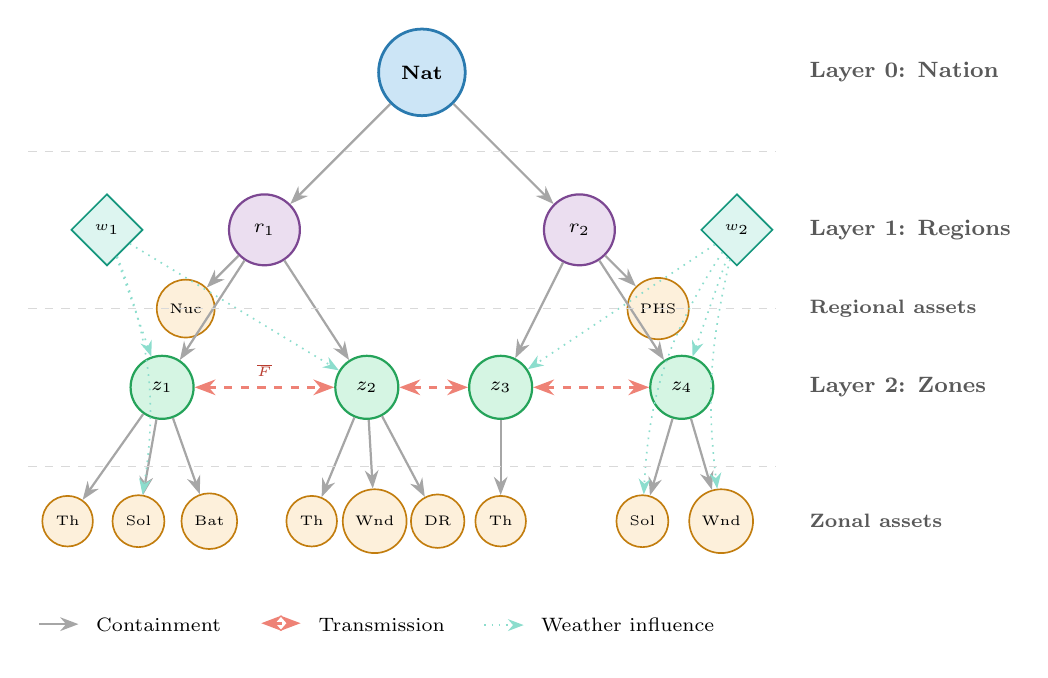
\begin{tikzpicture}[
    every node/.style={font=\small},
    nation/.style={circle, draw=scenarioBlue!80!black, fill=scenarioBlue!25, minimum size=1.1cm, line width=1pt, font=\scriptsize\bfseries},
    region/.style={circle, draw=encoderPurple!80!black, fill=encoderPurple!20, minimum size=0.9cm, line width=0.8pt, font=\scriptsize\bfseries},
    zone/.style={circle, draw=graphGreen!80!black, fill=graphGreen!20, minimum size=0.8cm, line width=0.8pt, font=\scriptsize},
    asset/.style={circle, draw=ebmOrange!80!black, fill=ebmOrange!15, minimum size=0.55cm, line width=0.6pt, font=\tiny},
    weather/.style={diamond, draw=samplerTeal!80!black, fill=samplerTeal!15, minimum size=0.7cm, line width=0.6pt, font=\tiny},
    contain/.style={->, >=Stealth, draw=gray!70, line width=0.8pt},
    trans/.style={<->, >=Stealth, draw=milpRed!70, line width=1pt, dashed},
    weath/.style={->, >=Stealth, draw=samplerTeal!50, line width=0.6pt, dotted},
    layerlabel/.style={font=\footnotesize\bfseries, text=gray!70!black},
]
\node[nation] (N) at (2.5, 6) {Nat};
\node[region] (R1) at (0.5, 4) {$r_1$};
\node[region] (R2) at (4.5, 4) {$r_2$};
\node[zone] (Z1) at (-0.8, 2) {$z_1$};
\node[zone] (Z2) at (1.8, 2) {$z_2$};
\node[zone] (Z3) at (3.5, 2) {$z_3$};
\node[zone] (Z4) at (5.8, 2) {$z_4$};
\node[asset] (A1th) at (-2.0, 0.3) {Th};
\node[asset] (A1sol) at (-1.1, 0.3) {Sol};
\node[asset] (A1bat) at (-0.2, 0.3) {Bat};
\node[asset] (A2th) at (1.1, 0.3) {Th};
\node[asset] (A2wnd) at (1.9, 0.3) {Wnd};
\node[asset] (A2dr) at (2.7, 0.3) {DR};
\node[asset] (A1nuc) at (-0.5, 3) {Nuc};
\node[asset] (A3th) at (3.5, 0.3) {Th};
\node[asset] (A2phs) at (5.5, 3) {PHS};
\node[asset] (A4sol) at (5.3, 0.3) {Sol};
\node[asset] (A4wnd) at (6.3, 0.3) {Wnd};
\node[weather] (W1) at (-1.5, 4) {$w_1$};
\node[weather] (W2) at (6.5, 4) {$w_2$};
\draw[contain] (N) -- (R1); \draw[contain] (N) -- (R2);
\draw[contain] (R1) -- (Z1); \draw[contain] (R1) -- (Z2);
\draw[contain] (R2) -- (Z3); \draw[contain] (R2) -- (Z4);
\draw[contain] (Z1) -- (A1th); \draw[contain] (Z1) -- (A1sol); \draw[contain] (Z1) -- (A1bat);
\draw[contain] (Z2) -- (A2th); \draw[contain] (Z2) -- (A2wnd); \draw[contain] (Z2) -- (A2dr);
\draw[contain] (R1) -- (A1nuc); \draw[contain] (R2) -- (A2phs);
\draw[contain] (Z3) -- (A3th); \draw[contain] (Z4) -- (A4sol); \draw[contain] (Z4) -- (A4wnd);
\draw[trans] (Z1) -- (Z2) node[midway, above, font=\tiny, text=milpRed!80!black] {$\overline{F}$};
\draw[trans] (Z2) -- (Z3); \draw[trans] (Z3) -- (Z4);
\draw[weath] (W1) -- (Z1); \draw[weath] (W1) -- (Z2); \draw[weath] (W1) to[bend left=15] (A1sol);
\draw[weath] (W2) -- (Z3); \draw[weath] (W2) -- (Z4); \draw[weath] (W2) to[bend right=15] (A4sol); \draw[weath] (W2) to[bend right=10] (A4wnd);
\node[layerlabel, anchor=west] at (7.3, 6) {Layer 0: Nation};
\node[layerlabel, anchor=west] at (7.3, 4) {Layer 1: Regions};
\node[layerlabel, anchor=west] at (7.3, 3) {\scriptsize Regional assets};
\node[layerlabel, anchor=west] at (7.3, 2) {Layer 2: Zones};
\node[layerlabel, anchor=west] at (7.3, 0.3) {\scriptsize Zonal assets};
\draw[gray!30, dashed] (-2.5, 5) -- (7, 5);
\draw[gray!30, dashed] (-2.5, 3) -- (7, 3);
\draw[gray!30, dashed] (-2.5, 1) -- (7, 1);
\node[anchor=north west] at (-2.5, -0.7) {
\begin{tabular}{@{}l@{\hspace{6pt}}l@{\hspace{14pt}}l@{\hspace{6pt}}l@{\hspace{14pt}}l@{\hspace{6pt}}l@{}}
\tikz\draw[contain] (0,0) -- (0.5,0); & \scriptsize Containment &
\tikz\draw[trans] (0,0) -- (0.5,0); & \scriptsize Transmission &
\tikz\draw[weath] (0,0) -- (0.5,0); & \scriptsize Weather influence \\
\end{tabular}
};
\end{tikzpicture}
}
\caption{Spatial structure of the multi-layer heterogeneous graph at a single time step. The containment hierarchy (nation $\to$ regions $\to$ zones) forms a tree; assets attach at the appropriate level---regional assets (nuclear, pumped hydro) are children of regions, while zonal assets (thermal, solar, wind, battery, DR) are children of zones. Bidirectional transmission edges connect zones, and weather influence edges reach zones and renewable assets.}
\label{fig:graph_spatial}
\end{figure}

\begin{figure}[htbp]
\centering
\resizebox{0.85\textwidth}{!}{%
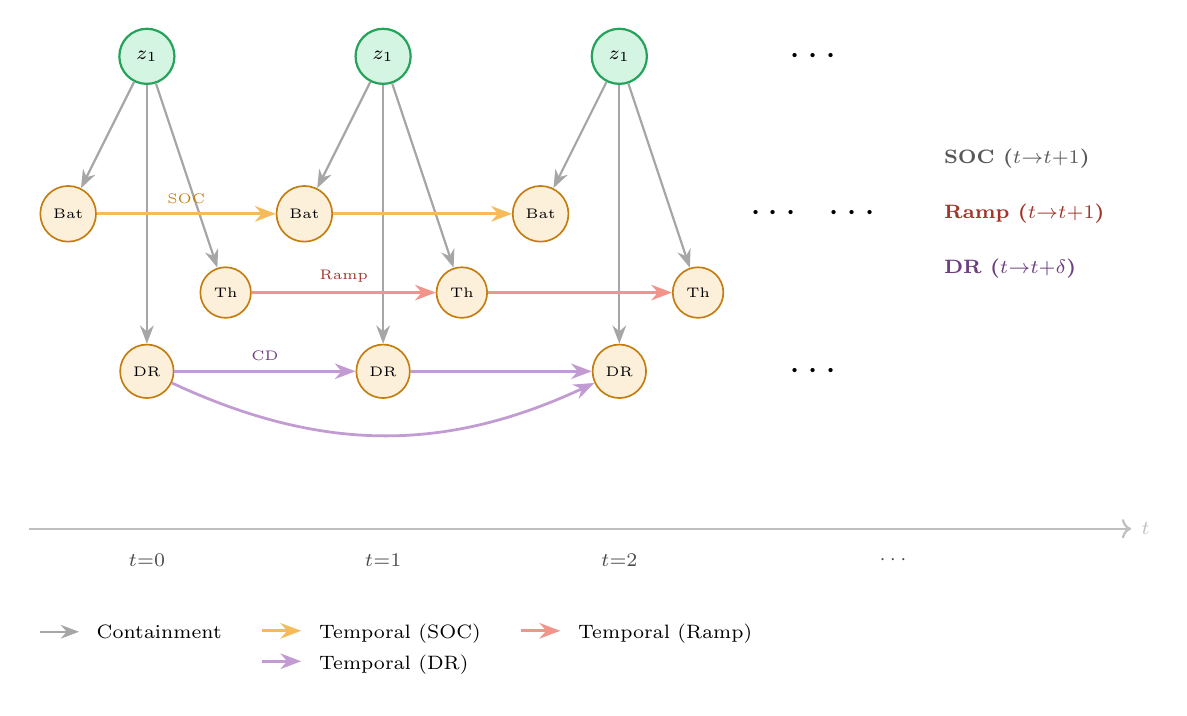
\begin{tikzpicture}[
    every node/.style={font=\small},
    zone/.style={circle, draw=graphGreen!80!black, fill=graphGreen!20, minimum size=0.8cm, line width=0.8pt, font=\scriptsize},
    asset/.style={circle, draw=ebmOrange!80!black, fill=ebmOrange!15, minimum size=0.55cm, line width=0.6pt, font=\tiny},
    contain/.style={->, >=Stealth, draw=gray!70, line width=0.8pt},
    temporal/.style={->, >=Stealth, draw=ebmOrange!70, line width=1pt},
    layerlabel/.style={font=\footnotesize\bfseries, text=gray!70!black},
    timelabel/.style={font=\scriptsize\itshape, text=gray!60!black},
]
\draw[->, gray!50, line width=0.8pt] (0, -0.5) -- (14, -0.5) node[right, font=\scriptsize] {$t$};
\node[timelabel] at (1.5, -0.9) {$t{=}0$};
\node[timelabel] at (4.5, -0.9) {$t{=}1$};
\node[timelabel] at (7.5, -0.9) {$t{=}2$};
\node[timelabel] at (11, -0.9) {$\cdots$};
\node[zone, minimum size=0.7cm] (Z1t0) at (1.5, 5.5) {$z_1$};
\node[asset, minimum size=0.55cm] (Batt0) at (0.5, 3.5) {Bat};
\node[asset, minimum size=0.55cm] (Tht0) at (2.5, 2.5) {Th};
\node[asset, minimum size=0.55cm] (DRt0) at (1.5, 1.5) {DR};
\draw[contain] (Z1t0) -- (Batt0); \draw[contain] (Z1t0) -- (Tht0); \draw[contain] (Z1t0) -- (DRt0);
\node[zone, minimum size=0.7cm] (Z1t1) at (4.5, 5.5) {$z_1$};
\node[asset, minimum size=0.55cm] (Batt1) at (3.5, 3.5) {Bat};
\node[asset, minimum size=0.55cm] (Tht1) at (5.5, 2.5) {Th};
\node[asset, minimum size=0.55cm] (DRt1) at (4.5, 1.5) {DR};
\draw[contain] (Z1t1) -- (Batt1); \draw[contain] (Z1t1) -- (Tht1); \draw[contain] (Z1t1) -- (DRt1);
\node[zone, minimum size=0.7cm] (Z1t2) at (7.5, 5.5) {$z_1$};
\node[asset, minimum size=0.55cm] (Batt2) at (6.5, 3.5) {Bat};
\node[asset, minimum size=0.55cm] (Tht2) at (8.5, 2.5) {Th};
\node[asset, minimum size=0.55cm] (DRt2) at (7.5, 1.5) {DR};
\draw[contain] (Z1t2) -- (Batt2); \draw[contain] (Z1t2) -- (Tht2); \draw[contain] (Z1t2) -- (DRt2);
\draw[temporal] (Batt0) -- (Batt1) node[midway, above, font=\tiny, text=ebmOrange!80!black] {SOC};
\draw[temporal] (Batt1) -- (Batt2);
\draw[temporal, draw=milpRed!60] (Tht0) -- (Tht1) node[midway, above, font=\tiny, text=milpRed!70!black] {Ramp};
\draw[temporal, draw=milpRed!60] (Tht1) -- (Tht2);
\draw[temporal, draw=encoderPurple!60] (DRt0) -- (DRt1) node[midway, above, font=\tiny, text=encoderPurple!70!black] {CD};
\draw[temporal, draw=encoderPurple!60] (DRt0) to[bend right=25] (DRt2);
\draw[temporal, draw=encoderPurple!60] (DRt1) -- (DRt2);
\node at (10, 5.5) {\Large$\cdots$};
\node at (9.5, 3.5) {\Large$\cdots$};
\node at (10.5, 3.5) {\Large$\cdots$};
\node at (10, 1.5) {\Large$\cdots$};
\node[layerlabel, anchor=west] at (11.5, 4.2) {\scriptsize SOC ($t{\to}t{+}1$)};
\node[layerlabel, anchor=west, text=milpRed!70!black] at (11.5, 3.5) {\scriptsize Ramp ($t{\to}t{+}1$)};
\node[layerlabel, anchor=west, text=encoderPurple!70!black] at (11.5, 2.8) {\scriptsize DR ($t{\to}t{+}\delta$)};
\node[anchor=north west] at (0, -1.5) {
\begin{tabular}{@{}l@{\hspace{6pt}}l@{\hspace{14pt}}l@{\hspace{6pt}}l@{\hspace{14pt}}l@{\hspace{6pt}}l@{}}
\tikz\draw[contain] (0,0) -- (0.5,0); & \scriptsize Containment &
\tikz\draw[temporal] (0,0) -- (0.5,0); & \scriptsize Temporal (SOC) &
\tikz\draw[temporal, draw=milpRed!60] (0,0) -- (0.5,0); & \scriptsize Temporal (Ramp) \\
& & \tikz\draw[temporal, draw=encoderPurple!60] (0,0) -- (0.5,0); & \scriptsize Temporal (DR) & & \\
\end{tabular}
};
\end{tikzpicture}
}
\caption{Temporal extension of the heterogeneous graph into a supra-graph, illustrated for a single zone~$z_1$ with three asset types. Each base node is replicated at every time step. Inter-temporal edges encode MILP coupling constraints: SOC continuity on storage assets (battery), ramping limits on thermal generators, and multi-step demand-response cooldown edges ($\delta \in \{1, \dots, \Delta_{\mathrm{cd}}\}$).}
\label{fig:graph_temporal}
\end{figure}

\subsection{Hierarchical Temporal Encoder: architecture and training details}
\label{app:hte_details}

\subsubsection*{Input projection}

Each supra-node feature vector $x^{\mathrm{supra}}_{(v,t)} \in \mathbb{R}^{d_{\max} + F_t}$ is projected to hidden dimension $D$:
\begin{equation}
h^{(0)}_{v,t} = W_{\mathrm{in}}\, x^{\mathrm{supra}}_{(v,t)} + b_{\mathrm{in}}, \qquad W_{\mathrm{in}} \in \mathbb{R}^{D \times (d_{\max}+F_t)}.
\end{equation}
The result is reshaped into $H^{(0)} \in \mathbb{R}^{N_{\mathrm{base}} \times T \times D}$.

\subsubsection*{Phase~1: Bottom-up spatial encoding}

At each level $\ell \in \{\text{asset}, \text{zone}, \text{region}\}$, $L_s$ GATv2 layers~\citep{brody_how_2022} ($H$ heads, $D/H$ dim per head, no concatenation) update representations via:
\begin{equation}
\tilde{h}^{(l)} = \mathrm{GATv2}\!\bigl(h^{(l-1)},\, \mathcal{E}_\ell\bigr), \quad
h^{(l)} = h^{(l-1)} + \mathrm{Dropout}\!\bigl(\mathrm{GELU}\!\bigl(\mathrm{LayerNorm}(\tilde{h}^{(l)})\bigr)\bigr).
\label{eq:gat_block}
\end{equation}
Edge sets $\mathcal{E}_\ell$: full supra-graph at asset level, intra-region FC at zone level, all-to-all at region level. After each block, a skip connection is saved and mean-pooling aggregates to the next coarser level:
\begin{equation}
h^{\mathrm{pool}}_{c,t} = \frac{1}{|\pi^{-1}(c)|} \sum_{v \in \pi^{-1}(c)} h^{(L_s)}_{v,t}.
\label{eq:pool}
\end{equation}
A final mean over regions yields $H_{\mathrm{nat}} \in \mathbb{R}^{1 \times T \times D}$.

\subsubsection*{Phase~2: Temporal Transformer}

A Transformer encoder~\citep{vaswani2017attention} ($L_t$ layers, $H$ heads, FFN width $4D$, sinusoidal positional encoding):
\begin{equation}
H^{\mathrm{temp}}_{\mathrm{nat}} = \mathrm{TransformerEncoder}\!\bigl(\mathrm{PosEnc}(H_{\mathrm{nat}})\bigr) \in \mathbb{R}^{1 \times T \times D}.
\label{eq:temporal_transformer}
\end{equation}

\subsubsection*{Phase~3: Top-down decoding}

Skip connections and GATv2 decoders propagate the nation representation back:
\begin{align}
H^{\mathrm{dec}}_{\mathrm{reg}} &= \mathrm{GATv2}_{\mathrm{reg}}^{\mathrm{dec}}\!\Bigl(\mathrm{broadcast}(H^{\mathrm{temp}}_{\mathrm{nat}}) + H^{\mathrm{skip}}_{\mathrm{reg}}\Bigr), \label{eq:topdown_reg} \\
H^{\mathrm{dec}}_{\mathrm{zon}} &= \mathrm{GATv2}_{\mathrm{zon}}^{\mathrm{dec}}\!\Bigl(\mathrm{unpool}_{\pi_{\mathrm{z \to r}}}(H^{\mathrm{dec}}_{\mathrm{reg}}) + H^{\mathrm{skip}}_{\mathrm{zon}}\Bigr), \label{eq:topdown_zon} \\
H^{\mathrm{dec}}_{\mathrm{ast}} &= \mathrm{GATv2}_{\mathrm{ast}}^{\mathrm{dec}}\!\Bigl(\mathrm{unpool}_{\pi_{\mathrm{a \to z}}}(H^{\mathrm{dec}}_{\mathrm{zon}}) + H^{\mathrm{skip}}_{\mathrm{ast}}\Bigr), \label{eq:topdown_ast}
\end{align}
where $h^{\mathrm{unpool}}_{v,t} = h^{\mathrm{dec}}_{\pi(v),t}$ indexes into the parent embedding.

\subsubsection*{Output}

\begin{equation}
\mathrm{HTE}(s) = \bigl\{
  H_{\mathrm{ast}} \!\in\! \mathbb{R}^{N_a \times T \times D},\;
  H_{\mathrm{zon}} \!\in\! \mathbb{R}^{N_z \times T \times D},\;
  H_{\mathrm{reg}} \!\in\! \mathbb{R}^{N_r \times T \times D},\;
  H_{\mathrm{nat}} \!\in\! \mathbb{R}^{T \times D}
\bigr\}.
\label{eq:hte_output}
\end{equation}

\subsubsection*{Multi-lag InfoNCE loss}

Anchor--positive pairs at lags $\Lambda = \{1, 4, 8\}$ on $\ell_2$-normalised asset embeddings:
\begin{equation}
\mathcal{L}_{\mathrm{NCE}} = -\frac{1}{|\mathcal{P}|} \sum_{(a,p) \in \mathcal{P}} \log \frac{\exp(\mathrm{sim}(a, p) / \kappa)}{\exp(\mathrm{sim}(a, p) / \kappa) + \sum_{j=1}^{M_{\mathrm{neg}}} \exp(\mathrm{sim}(a, n_j) / \kappa)},
\label{eq:infonce}
\end{equation}
where $\mathrm{sim}(a, b) = a^\top b / (\|a\|\|b\|)$ and $\kappa$ is a temperature parameter.

\subsubsection*{Hyperparameters}

\begin{table}[htbp]
\centering
\small
\begin{tabular}{lll}
\toprule
\textbf{Category} & \textbf{Hyperparameter} & \textbf{Value} \\
\midrule
\multirow{4}{*}{Architecture}
  & Hidden dimension $D$ & 128 \\
  & Spatial GATv2 layers $L_s$ (per level) & 2 \\
  & Temporal Transformer layers $L_t$ & 4 \\
  & Attention heads $H$ & 8 \\
\midrule
\multirow{3}{*}{Loss}
  & Positive lags $\Lambda$ & $\{1, 4, 8\}$ \\
  & Temperature $\kappa$ (train / val) & 0.10 / 0.20 \\
  & Negative sample ratio & 0.25 / 0.10 \\
\midrule
\multirow{5}{*}{Optimisation}
  & Optimiser & AdamW \\
  & Learning rate (initial / max) & $1.5 \times 10^{-4}$ / $1.8 \times 10^{-4}$ \\
  & LR schedule & Cosine + 10-epoch warmup \\
  & Gradient accumulation & 8 steps \\
  & Early stopping patience & 10 epochs \\
\bottomrule
\end{tabular}
\caption{Hyperparameter configuration for the Hierarchical Temporal Encoder.}
\label{tab:hte_hyperparams}
\end{table}

\begin{figure}[htbp]
\centering
\resizebox{0.95\textwidth}{!}{%
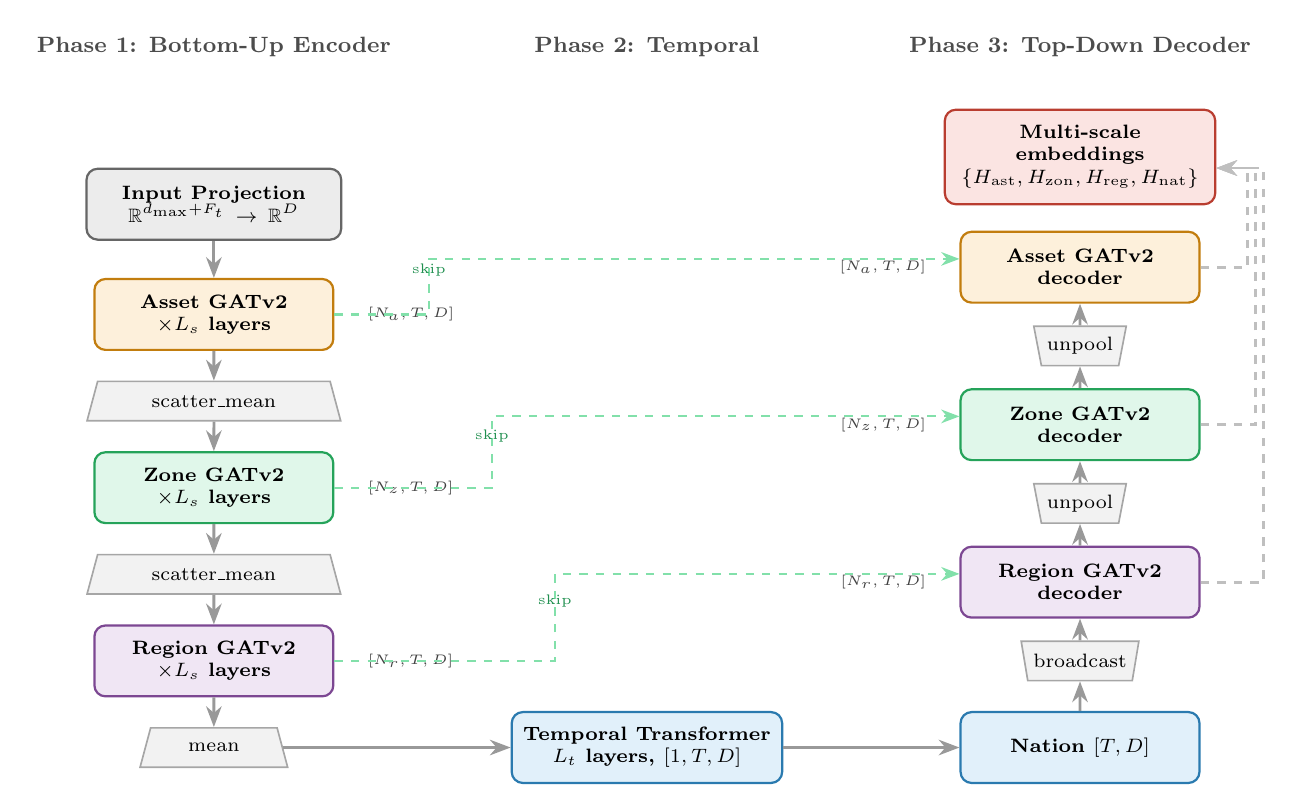
\begin{tikzpicture}[
    every node/.style={font=\small},
    block/.style={rectangle, rounded corners=4pt, draw=#1!80!black, fill=#1!15, minimum height=0.9cm, text width=2.8cm, align=center, font=\scriptsize\bfseries, line width=0.8pt},
    pool/.style={trapezium, trapezium angle=75, draw=gray!70, fill=gray!10, minimum height=0.5cm, font=\tiny, align=center, line width=0.6pt, inner sep=2pt},
    unpool/.style={trapezium, trapezium angle=75, trapezium stretches body, draw=gray!70, fill=gray!10, minimum height=0.5cm, font=\tiny, align=center, line width=0.6pt, inner sep=2pt, shape border rotate=180},
    skip/.style={->, >=Stealth, draw=graphGreen!60, line width=0.8pt, dashed},
    flow/.style={->, >=Stealth, draw=gray!80, line width=1pt},
    phaselabel/.style={font=\footnotesize\bfseries, text=gray!60!black},
    dimlab/.style={font=\tiny\itshape, text=gray!50!black},
]
% PHASE 1
\node[phaselabel] at (0, 8.2) {Phase 1: Bottom-Up Encoder};
\node[block=gray, text width=3cm] (input) at (0, 6.2) {Input Projection\\$\mathbb{R}^{d_{\max}+F_t} \to \mathbb{R}^D$};
\node[block=ebmOrange] (asset_gat) at (0, 4.8) {Asset GATv2\\$\times L_s$ layers};
\node[dimlab, right=0.3cm of asset_gat] {$[N_a, T, D]$};
\node[pool] (pool_az) at (0, 3.7) {\scriptsize scatter\_mean};
\node[block=graphGreen] (zone_gat) at (0, 2.6) {Zone GATv2\\$\times L_s$ layers};
\node[dimlab, right=0.3cm of zone_gat] {$[N_z, T, D]$};
\node[pool] (pool_zr) at (0, 1.5) {\scriptsize scatter\_mean};
\node[block=encoderPurple] (region_gat) at (0, 0.4) {Region GATv2\\$\times L_s$ layers};
\node[dimlab, right=0.3cm of region_gat] {$[N_r, T, D]$};
\node[pool] (pool_rn) at (0, -0.7) {\scriptsize mean};
\draw[flow] (input) -- (asset_gat);
\draw[flow] (asset_gat) -- (pool_az);
\draw[flow] (pool_az) -- (zone_gat);
\draw[flow] (zone_gat) -- (pool_zr);
\draw[flow] (pool_zr) -- (region_gat);
\draw[flow] (region_gat) -- (pool_rn);
% PHASE 2
\node[phaselabel] at (5.5, 8.2) {Phase 2: Temporal};
\node[block=scenarioBlue, text width=3.2cm] (temporal) at (5.5, -0.7) {Temporal Transformer\\$L_t$ layers, $[1, T, D]$};
\draw[flow] (pool_rn) -- (temporal);
% PHASE 3
\node[phaselabel] at (11, 8.2) {Phase 3: Top-Down Decoder};
\node[block=scenarioBlue, text width=2.8cm] (nat_out) at (11, -0.7) {Nation $[T, D]$};
\draw[flow] (temporal) -- (nat_out);
\node[unpool] (unpool_nr) at (11, 0.4) {\scriptsize broadcast};
\node[block=encoderPurple] (region_dec) at (11, 1.4) {Region GATv2\\decoder};
\node[dimlab, left=0.3cm of region_dec] {$[N_r, T, D]$};
\node[unpool] (unpool_rz) at (11, 2.4) {\scriptsize unpool};
\node[block=graphGreen] (zone_dec) at (11, 3.4) {Zone GATv2\\decoder};
\node[dimlab, left=0.3cm of zone_dec] {$[N_z, T, D]$};
\node[unpool] (unpool_za) at (11, 4.4) {\scriptsize unpool};
\node[block=ebmOrange] (asset_dec) at (11, 5.4) {Asset GATv2\\decoder};
\node[dimlab, left=0.3cm of asset_dec] {$[N_a, T, D]$};
\draw[flow] (nat_out.north) -- (unpool_nr.south);
\draw[flow] (unpool_nr) -- (region_dec);
\draw[flow] (region_dec) -- (unpool_rz);
\draw[flow] (unpool_rz) -- (zone_dec);
\draw[flow] (zone_dec) -- (unpool_za);
\draw[flow] (unpool_za) -- (asset_dec);
% SKIP CONNECTIONS
\draw[skip] (asset_gat.east) -- ++(1.2,0) |- ([yshift=3pt]asset_dec.west) node[pos=0.25, above, font=\tiny, text=graphGreen!70!black] {skip};
\draw[skip] (zone_gat.east) -- ++(2.0,0) |- ([yshift=3pt]zone_dec.west) node[pos=0.25, above, font=\tiny, text=graphGreen!70!black] {skip};
\draw[skip] (region_gat.east) -- ++(2.8,0) |- ([yshift=3pt]region_dec.west) node[pos=0.25, above, font=\tiny, text=graphGreen!70!black] {skip};
% OUTPUT
\node[block=milpRed, text width=3.2cm, minimum height=1.2cm] (output) at (11, 6.8) {Multi-scale embeddings\\$\{H_{\mathrm{ast}}, H_{\mathrm{zon}}, H_{\mathrm{reg}}, H_{\mathrm{nat}}\}$};
\draw[flow, dashed, draw=gray!50] (asset_dec.east) -- ++(0.6,0) |- ([yshift=-4pt]output.east);
\draw[flow, dashed, draw=gray!50] (zone_dec.east) -- ++(0.7,0) |- ([yshift=-4pt]output.east);
\draw[flow, dashed, draw=gray!50] (region_dec.east) -- ++(0.8,0) |- ([yshift=-4pt]output.east);
\end{tikzpicture}
}
\caption{Architecture of the Hierarchical Temporal Encoder (HTE). \textbf{Phase~1} (left): bottom-up spatial encoding with GATv2 convolutions, interspersed with mean-pooling steps following the containment hierarchy. \textbf{Phase~2} (centre): dense Transformer encoder on the nation-level sequence ($1 \times T$ tokens). \textbf{Phase~3} (right): top-down decoding via unpooling and GATv2 decoders, with skip connections (dashed green) preserving local spatial detail.}
\label{fig:hte_architecture}
\end{figure}

\end{document}
